%% =====================================================================
%% Generative AI, Assignment 1: technical report (IEEE conference format)
%% Eman Ul Huda (23i-2559). Compile with pdfLaTeX.
%% Application screenshots and the W&B screenshot are included automatically when
%% figures/app_universal.png, app_hard.png, app_soft.png, app_sketch.png and figures/wandb.png exist.
%% =====================================================================
\documentclass[conference]{IEEEtran}
\IEEEoverridecommandlockouts

\usepackage{cite}
\usepackage{amsmath,amssymb,amsfonts}
\usepackage{graphicx}
\usepackage{booktabs}
\usepackage{multirow}
\usepackage{array}
\usepackage{xcolor}
\usepackage{tikz}
\usetikzlibrary{positioning,arrows.meta,fit,calc}
\usepackage[hidelinks]{hyperref}

\graphicspath{{figures/}}

% Paste the YouTube link of the demonstration video between the braces; the report shows it automatically.
\newcommand*{\videourl}{https://youtu.be/B2mOOliPXoI}
\newcommand{\videosentence}{\ifx\videourl\empty\else The demonstration video is available at \url{\videourl}.\fi}

\begin{document}

\title{Generative Models for Multi-Corruption Image Restoration and Style-Conditioned Face-to-Sketch Synthesis}

\author{\IEEEauthorblockN{Eman Ul Huda}
\IEEEauthorblockA{Student ID 23i-2559 \\
Department of Computer Science \\
FAST National University of Computer and Emerging Sciences (FAST-NUCES)}}

\maketitle

% =====================================================================
\begin{abstract}
This report presents four related generative systems developed, evaluated and deployed as one browser-based application. Tasks 1 to 3 restore 128$\times$128 Oxford-IIIT Pet images affected by salt-and-pepper noise, Gaussian blur or rectangular occlusion: a universal denoising autoencoder (Task 1), a corruption classifier with hard-routed specialist autoencoders (Task 2), and a jointly trained soft mixture of experts (Task 3). On the official test set the universal autoencoder reaches an SSIM of 0.704, and hard routing reaches 0.735 with a classifier accuracy of 99.86\%, its gain coming mainly from passing clean images through unchanged. The jointly trained soft mixture of experts raises validation SSIM from 0.783 for hard routing to 0.839 by learning to blend the unchanged input with the experts according to how severe the damage is. Task 4 is a style-conditioned conditional GAN that translates face photographs into sketches in one of three FS2K artist styles, using a U-Net generator, a PatchGAN discriminator and a learned style embedding injected into both networks. On the official FS2K test set it reaches an SSIM of 0.463, an LPIPS of 0.211 and an FID of 37.6, and the true style condition produces the perceptually closest sketch for 72.9\% to 95.7\% of photographs depending on the style. All models were tuned with Optuna, tracked with Weights \& Biases, exported to ONNX and served through a FastAPI backend and a React interface running in Docker containers.
\end{abstract}

\begin{IEEEkeywords}
denoising autoencoder, mixture of experts, conditional GAN, image-to-image translation, facial sketch synthesis, Optuna, ONNX
\end{IEEEkeywords}

% =====================================================================
\section{Introduction}
Image restoration and image-to-image translation are two common uses of generative models. Restoration recovers a clean image from a corrupted observation; translation maps an image from one visual domain to another while keeping its content. This assignment studies both problems and asks how architectural choices (one shared model, hard routing to specialists, or soft weighting of specialists) and training objectives (pixel, structural, perceptual and adversarial losses) affect quality.

The contributions of this work are: (i) a universal restoration autoencoder trained on runtime-generated corruptions; (ii) a hard-routing system combining a corruption classifier with three specialist autoencoders, evaluated with oracle and predicted routing; (iii) a differentiable soft mixture of experts initialised from the Task 2 components and fine-tuned jointly; (iv) a style-conditioned conditional GAN for face-to-sketch generation; and (v) a containerised web application exposing all four systems. A central finding of Tasks 1 and 2 is that the bottleneck, not the routing, limits restoration quality, so deciding when not to restore matters as much as restoring well. The soft mixture of experts confirms this: without being told, its gate learned to keep most of a lightly corrupted input and to rely on an expert only as the damage grows.

The source code is available at \url{https://github.com/eman-huda/genai-assignment1}. \videosentence

% =====================================================================
\section{Related Work}
\textbf{Denoising autoencoders and restoration.} Denoising autoencoders learn robust representations by reconstructing clean inputs from corrupted ones \cite{vincent2008}. Convolutional encoder-decoders with skip connections are widely used for restoration \cite{mao2016}, and residual CNNs such as DnCNN handle blind Gaussian denoising \cite{zhang2017dncnn}. Context encoders address large missing regions \cite{pathak2016}. All-in-one restoration models handle several unknown degradations with a single network \cite{li2022airnet}, which is the setting of Task 1.

\textbf{Mixtures of experts.} Mixtures of experts combine specialised sub-networks through a gating network \cite{jacobs1991}. Sparse gating scales this idea to very large models \cite{shazeer2017}, and auxiliary load-balancing losses prevent the gate from collapsing onto a few experts \cite{shazeer2017,fedus2022}. Task 3 uses a dense softmax gate with a balance regulariser of this kind.

\textbf{Conditional GANs and sketch synthesis.} GANs train a generator against a discriminator \cite{goodfellow2014}; conditional GANs feed side information to both \cite{mirza2014}. Pix2pix combines a U-Net generator \cite{ronneberger2015}, a PatchGAN discriminator and an L1 term for paired translation \cite{isola2017}. Early face sketch synthesis relied on patch-based exemplar methods \cite{wang2009}. FS2K is the largest public facial sketch dataset with artist-drawn sketches in three styles; its authors' FSGAN conditions on style by expanding a style vector into a spatial map \cite{fan2022}, the approach adopted in Task 4. Projection discriminators are an alternative way to condition the discriminator on a class \cite{miyato2018proj}.

\textbf{Evaluation.} SSIM measures structural similarity \cite{wang2004}, LPIPS measures perceptual distance with deep features \cite{zhang2018lpips}, and FID compares distributions of Inception features \cite{heusel2017}. FID is biased for small sample sizes \cite{chong2020}, which motivates the Kernel Inception Distance (KID) \cite{binkowski2018}.

\textbf{Hyperparameter optimisation.} Optuna provides define-by-run search with pruning \cite{akiba2019}; its default sampler is the Tree-structured Parzen Estimator \cite{bergstra2011}, and parameter importances are estimated with fANOVA \cite{hutter2014}.

% =====================================================================
\section{Datasets and Preprocessing}

\subsection{Oxford-IIIT Pet with runtime corruptions (Tasks 1 to 3)}
The Oxford-IIIT Pet dataset \cite{parkhi2012} contains images of 37 cat and dog breeds; class labels are not used. The official trainval set was split 80/20 into training and validation sets with seed 42 (2,944 training and 736 validation images), and the official test set (3,669 images) was used only for final evaluation. All images were converted to RGB and resized to 128$\times$128. The same split is used for Tasks 1, 2 and 3.

During training, each loaded image receives one of four conditions with equal probability, sampled again every time the image is loaded (Table~\ref{tab:corruptions}). Validation corruptions are fixed in a manifest that stores the type, severity, random seed, blur settings and rectangle coordinates of every image. The test manifest contains each test image ten times: once clean and three fixed severities for each corruption. Rectangles are placed until their union reaches the target coverage within a small tolerance; across the test manifest the achieved occlusion coverage averaged 10.0\% (range 9.8\% to 10.3\%), 19.8\% (18.5\% to 20.5\%) and 34.5\% (33.5\% to 35.7\%) for the three levels. The validation manifest holds 184 images of each condition. Fig.~\ref{fig:corruption_examples} shows one image under every test level.

\begin{table}[t]
\centering
\caption{Corruption configuration (Tasks 1 to 3).}
\label{tab:corruptions}
\footnotesize
\setlength{\tabcolsep}{3pt}
\begin{tabular}{@{}p{1.3cm}p{3.2cm}p{2.95cm}@{}}
\toprule
Condition & Training (sampled per load) & Test levels (low / med / high) \\
\midrule
Clean & No corruption & n/a \\
Salt-and-pepper & $p \sim U(0.02, 0.15)$, black or white with equal probability & $p = 0.03 / 0.08 / 0.15$ \\
Gaussian blur & $k \in \{3,5,7\}$, $\sigma \sim U(0.5, 2.5)$ & $(3,0.7) / (5,1.5) / (7,2.5)$ \\
Occlusion & 1 to 3 black rectangles, union covers 10\% to 35\% & 1 / 2 / 3 rectangles, $\approx$10\% / 20\% / 35\% \\
\bottomrule
\end{tabular}
\end{table}

\begin{figure*}[t]
\centering
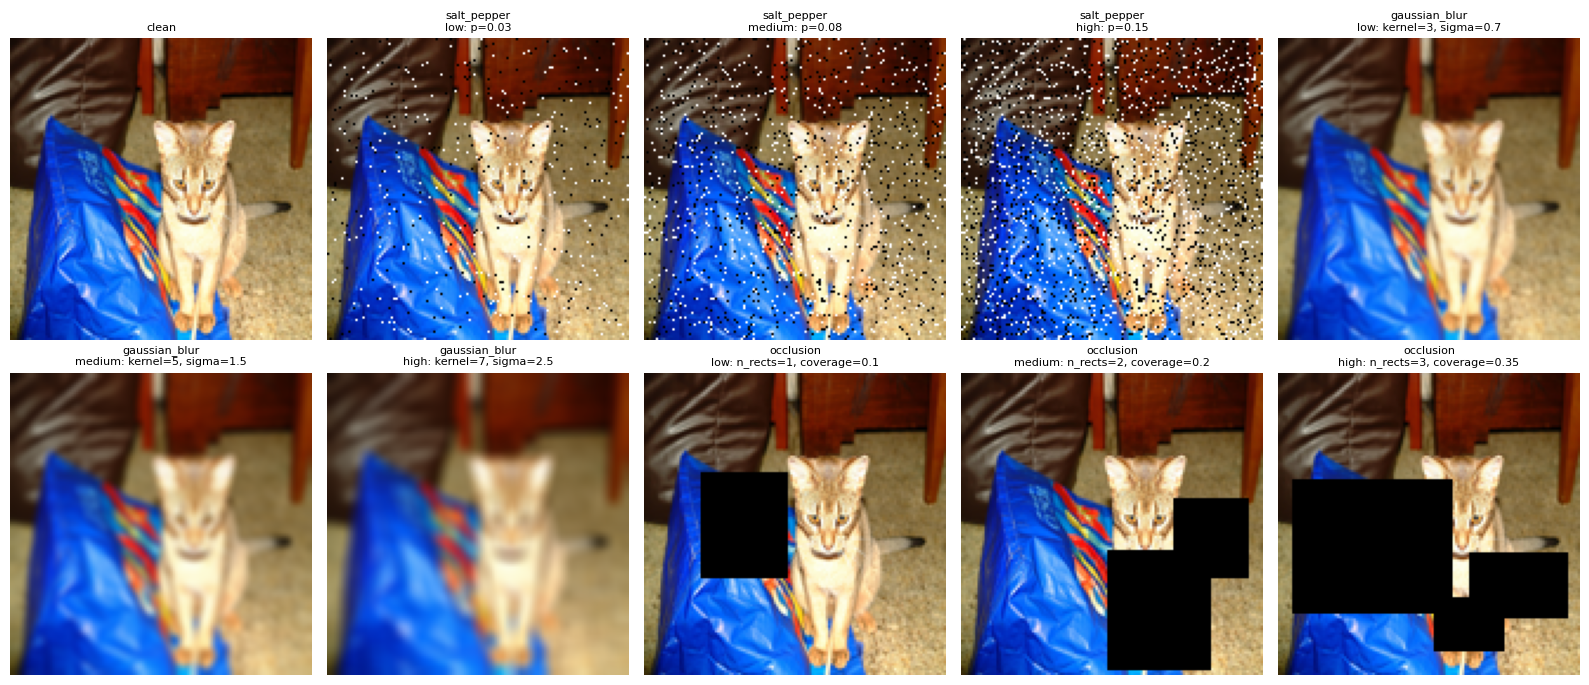
\includegraphics[width=0.92\textwidth]{t1_gallery.png}
\caption{One validation image under every fixed test level: clean, salt-and-pepper ($p$ = 0.03, 0.08, 0.15), Gaussian blur (kernel and $\sigma$ = (3, 0.7), (5, 1.5), (7, 2.5)) and occlusion (1, 2, 3 rectangles covering about 10\%, 20\%, 35\%).}
\label{fig:corruption_examples}
\end{figure*}

\subsection{FS2K (Task 4)}
FS2K contains 2,104 photograph-sketch pairs drawn by professional artists in three styles \cite{fan2022}: 1,058 pairs in the official training set and 1,046 in the official test set. The official definitions were kept. A validation set of 15\% of the official training portion was drawn with seed 42, stratified by style (Table~\ref{tab:fs2k_split}). The official test set was used only once, for the final evaluation.

\begin{table}[t]
\centering
\caption{FS2K splits used in Task 4 (pairs per style).}
\label{tab:fs2k_split}
\footnotesize
\begin{tabular}{@{}lrrrr@{}}
\toprule
Split & Style 1 & Style 2 & Style 3 & Total \\
\midrule
Training (85\% of official train) & 303 & 298 & 298 & 899 \\
Validation (15\%, stratified) & 54 & 52 & 53 & 159 \\
Test (official) & 619 & 381 & 46 & 1,046 \\
\bottomrule
\end{tabular}
\end{table}

Each annotation entry was matched to its files using the naming rule of the authors' split script (photo \texttt{photo1/image0110} corresponds to sketch \texttt{sketch1/sketch0110}). All 2,104 pairs were found, with no missing files and no size mismatch between a photograph and its sketch. Images were converted to RGB (greyscale images were expanded and transparent images composited on white), resized to 128$\times$128 with area interpolation, and scaled to $[-1, 1]$.

Training augmentation follows pix2pix \cite{isola2017}: both images are resized to 142$\times$142, cropped back to 128$\times$128 at the same random offset, and flipped horizontally together with probability 0.5. Applying one sampled transformation to both images preserves the pixel correspondence that paired training relies on; Fig.~\ref{fig:t4_aug} confirms visually that the augmented photograph and sketch remain aligned.

Fig.~\ref{fig:t4_data} shows that the three styles differ mainly in stroke weight and shading. Style 1 uses light, thin outlines with little shading; Style 2 uses dark, heavy strokes and dense hatching, especially in the hair; Style 3 lies between the two, with moderate shading and more facial detail. The official test set is strongly imbalanced, with only 46 Style 3 pairs, which affects how reliable per-style test statistics are (Section~\ref{sec:t4_results}).

\begin{figure}[t]
\centering
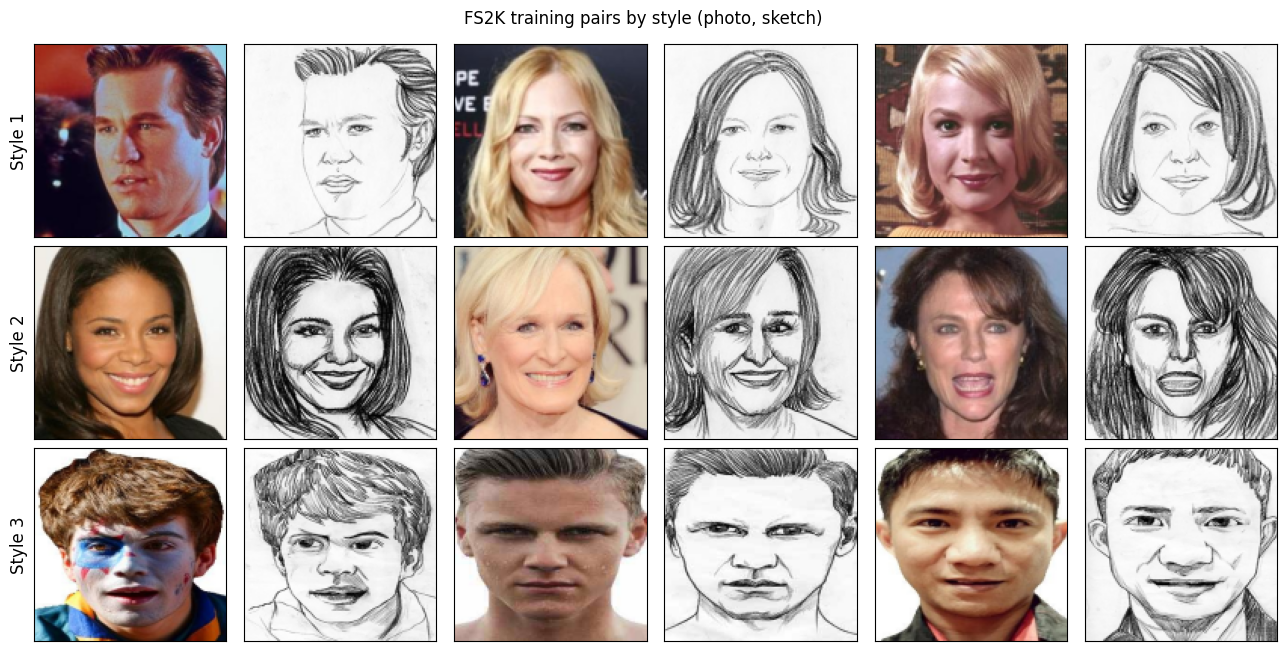
\includegraphics[width=\linewidth]{t4_dataset_examples.png}
\caption{FS2K training pairs, three per style (photograph left, sketch right).}
\label{fig:t4_data}
\end{figure}

\begin{figure}[t]
\centering
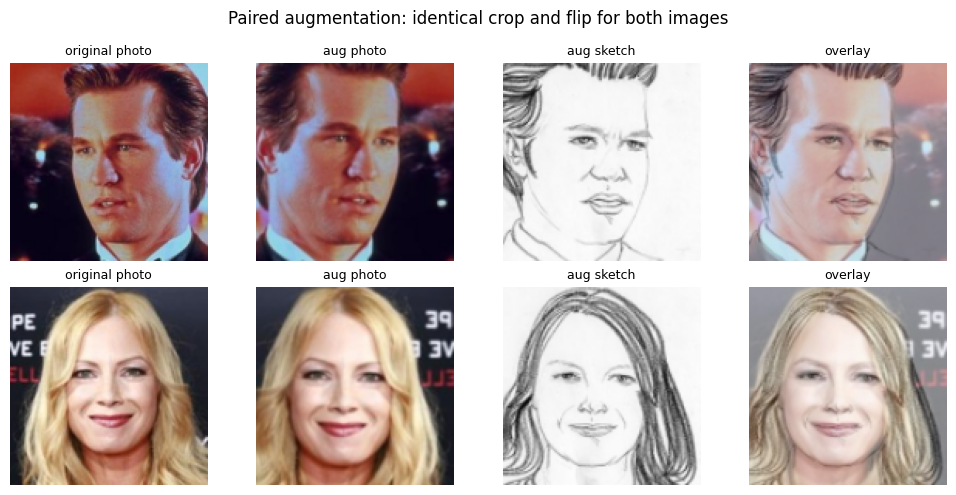
\includegraphics[width=0.9\linewidth]{t4_paired_augmentation.png}
\caption{Paired augmentation check: the overlay of the augmented photograph and sketch shows that both received the same crop and flip.}
\label{fig:t4_aug}
\end{figure}

% =====================================================================
\section{Task 1: Universal Multi-Corruption Denoising Autoencoder}

\subsection{Architecture}
The network is a convolutional autoencoder with a genuine bottleneck (Fig.~\ref{fig:t1_arch}). A stem of two 3$\times$3 convolutions (BatchNorm, ReLU) keeps the full 128$\times$128 resolution with $c$ channels. Four down-blocks, each a stride-2 convolution followed by a 3$\times$3 convolution, reduce the resolution to 64, 32, 16 and 8 while the channels grow to $2c, 4c, 8c, 8c$. A 1$\times$1 convolution then compresses the 8$\times$8 features to $L$ latent channels. The decoder mirrors the encoder: a 1$\times$1 convolution back to $8c$ channels and four up-blocks of bilinear upsampling followed by two convolutions, which avoids the checkerboard artefacts of transposed convolutions \cite{odena2016}. A 3$\times$3 convolution with a sigmoid outputs the RGB image. Spatial dropout follows every block.

Optuna selected $c = 48$ and $L = 64$, so the latent tensor has $64 \times 8 \times 8 = 4{,}096$ values: 8.3\% of the $3 \times 128 \times 128 = 49{,}152$ input values, a 12:1 compression. The model has 9,308,515 parameters. No skip connection bypasses the bottleneck, so every output pixel must be reconstructed from the latent code.

\begin{figure}[t]
\centering
\resizebox{\linewidth}{!}{%
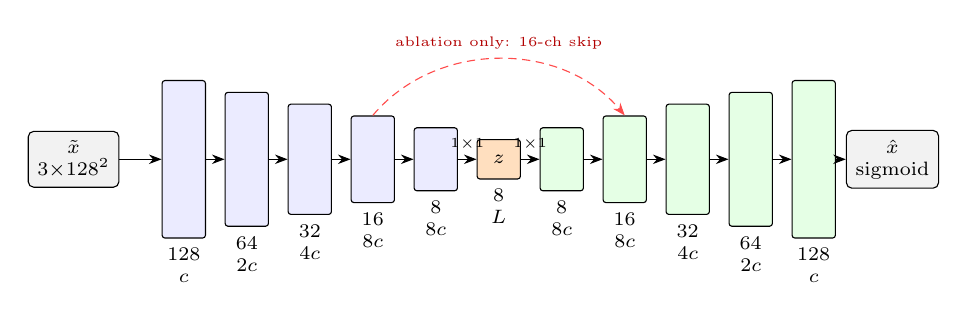
\begin{tikzpicture}[font=\scriptsize, >={Stealth[length=1.6mm]},
  enc/.style={draw, rounded corners=1pt, fill=blue!8, minimum width=0.55cm, align=center},
  dec/.style={draw, rounded corners=1pt, fill=green!10, minimum width=0.55cm, align=center},
  lat/.style={draw, rounded corners=1pt, fill=orange!25, minimum width=0.55cm, minimum height=0.5cm, align=center},
  io/.style={draw, rounded corners=2pt, fill=gray!10, align=center}]
\node[io] (in) at (0,0) {$\tilde{x}$\\$3{\times}128^2$};
\foreach \i/\h/\lab in {1/2.0/{128\\$c$}, 2/1.7/{64\\$2c$}, 3/1.4/{32\\$4c$}, 4/1.1/{16\\$8c$}, 5/0.8/{8\\$8c$}}{
  \node[enc, minimum height=\h cm] (e\i) at ({0.6+0.8*\i},0) {};
  \node[below=0pt of e\i, align=center] {\lab};
}
\node[lat] (z) at (5.4,0) {$z$};
\node[below=0pt of z, align=center] {8\\$L$};
\foreach \i/\h/\lab in {1/0.8/{8\\$8c$}, 2/1.1/{16\\$8c$}, 3/1.4/{32\\$4c$}, 4/1.7/{64\\$2c$}, 5/2.0/{128\\$c$}}{
  \node[dec, minimum height=\h cm] (d\i) at ({5.4+0.8*\i},0) {};
  \node[below=0pt of d\i, align=center] {\lab};
}
\node[io] (out) at (10.4,0) {$\hat{x}$\\sigmoid};
\draw[->] (in) -- (e1); \draw[->] (e1) -- (e2); \draw[->] (e2) -- (e3); \draw[->] (e3) -- (e4); \draw[->] (e4) -- (e5);
\draw[->] (e5) -- node[above]{\tiny 1$\times$1} (z); \draw[->] (z) -- node[above]{\tiny 1$\times$1} (d1);
\draw[->] (d1) -- (d2); \draw[->] (d2) -- (d3); \draw[->] (d3) -- (d4); \draw[->] (d4) -- (d5); \draw[->] (d5) -- (out);
\draw[->, red!70, densely dashed] (e4.north) to[out=50, in=130] node[above, text=red!70!black]{\tiny ablation only: 16-ch skip} (d2.north);
\end{tikzpicture}}
\caption{Task 1 autoencoder. Numbers give spatial size and channels ($c = 48$, $L = 64$). Strided-convolution encoder (blue), 1$\times$1 bottleneck (orange), upsampling decoder (green). The dashed skip was used only in the ablation of Section~\ref{sec:t1_skip}.}
\label{fig:t1_arch}
\end{figure}

\subsection{Loss function}
With clean image $x$, corrupted input $\tilde{x}$ and reconstruction $\hat{x} = D(E(\tilde{x}))$, the training loss is
\begin{equation}
\mathcal{L}_{\text{rec}} = \alpha\, \mathcal{L}_{1}(x, \hat{x}) + (1-\alpha)\,\bigl(1 - \text{SSIM}(x, \hat{x})\bigr).
\label{eq:t1_loss}
\end{equation}
The L1 term enforces pixel accuracy and the SSIM term \cite{wang2004} (11$\times$11 Gaussian window, $\sigma = 1.5$) preserves edges, local contrast and structure. The model is never told which corruption was applied.

\subsection{Training and hyperparameter optimisation}
\label{sec:t1_optuna}
Training uses Adam with the runtime corruption pipeline of Section~III: every loaded image receives a freshly sampled condition and severity. Optuna \cite{akiba2019} searched six hyperparameters (Table~\ref{tab:t1_optuna}) with the TPE sampler \cite{bergstra2011} and median pruning, using 25 trials of 8 epochs each. Trials were compared on the fixed validation objective $\text{L1} + (1-\text{SSIM})$, which does not depend on the tuned $\alpha$; otherwise a trial could improve its score by reweighting the metric rather than by restoring better.

\begin{table}[t]
\centering
\caption{Task 1 Optuna search space and selected values (best of 25 trials, 8 epochs each).}
\label{tab:t1_optuna}
\footnotesize
\begin{tabular}{@{}lll@{}}
\toprule
Hyperparameter & Search range & Selected \\
\midrule
Learning rate & log-uniform $[10^{-4}, 3\times10^{-3}]$ & $4.21\times10^{-4}$ \\
Batch size & $\{16, 32, 64\}$ & 16 \\
Latent channels $L$ & $\{8, 16, 32, 64\}$ & 64 \\
Base channels $c$ & $\{16, 32, 48\}$ & 48 \\
Dropout & uniform $[0, 0.3]$ & 0.219 \\
Loss weight $\alpha$ & uniform $[0.5, 0.95]$ & 0.508 \\
\midrule
Validation objective & & 0.4561 (trial 18) \\
\bottomrule
\end{tabular}
\end{table}

Of the 25 trials, 23 completed and 2 were pruned; the objective fell from 0.608 (trial 0) to 0.456 (trial 18) (Fig.~\ref{fig:t1_optuna}). Every competitive trial used $c = 48$ and batch size 16, and the two completed trials with the smallest latent ($L = 8$) scored 0.480 and 0.487, behind the best $L = 64$ trials (0.456 to 0.467). This shows that latent capacity limits quality. The fANOVA importances \cite{hutter2014} attribute 0.65 to dropout and 0.30 to $\alpha$; the categorical parameters receive almost none because TPE quickly concentrated on $c = 48$ and batch size 16, so their effect was not resolved rather than shown to be absent. Optuna also pushed $\alpha$ to the low end of its range (0.508), giving the SSIM term almost half the weight. The starting value of 0.8 suggested in the brief would have favoured pixel accuracy over structure.

\begin{figure}[t]
\centering
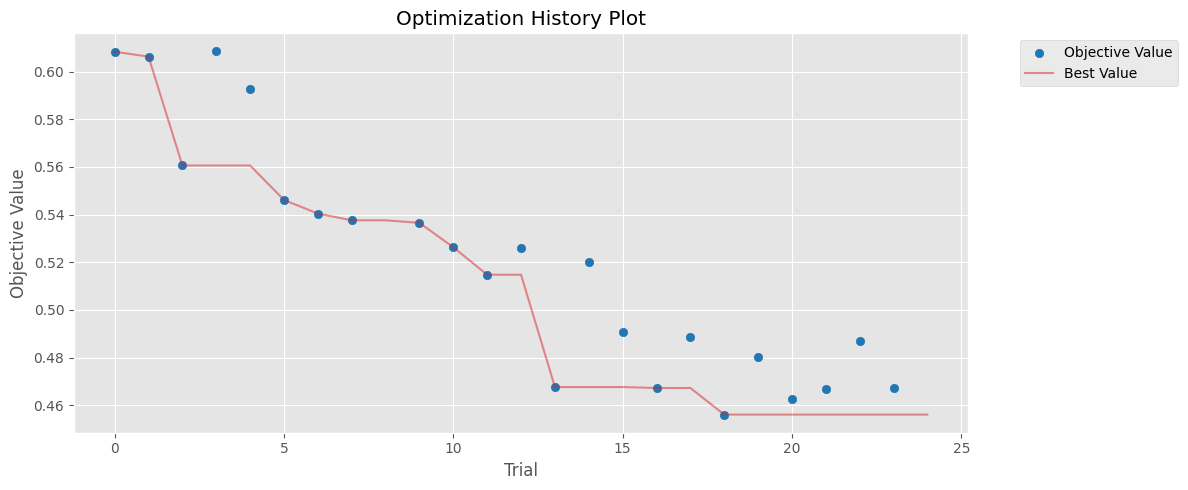
\includegraphics[width=0.95\linewidth]{t1_optuna_history.png}\\[2pt]
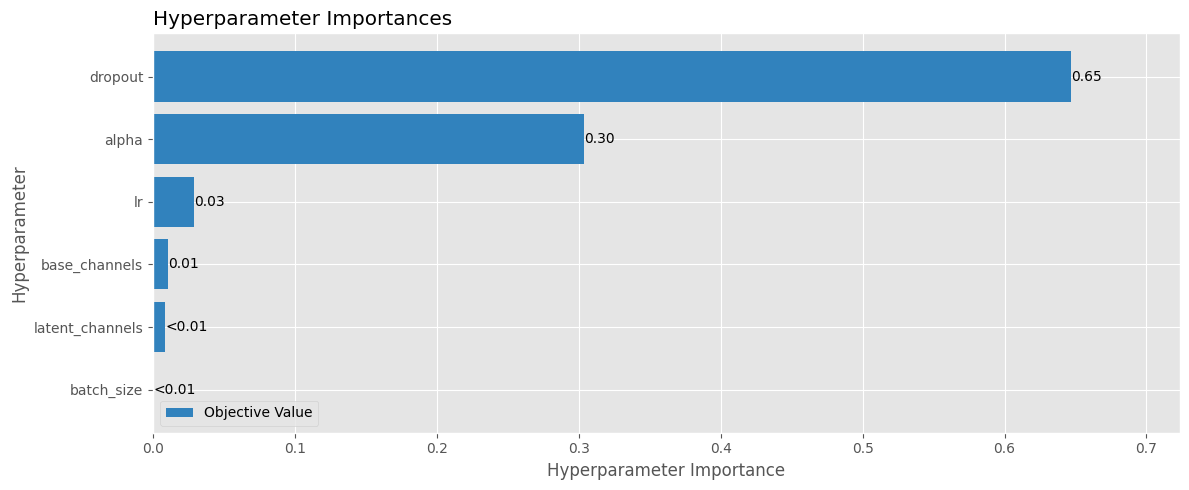
\includegraphics[width=0.95\linewidth]{t1_optuna_importance.png}
\caption{Task 1 Optuna study: objective per trial (top) and fANOVA importance over completed trials (bottom).}
\label{fig:t1_optuna}
\end{figure}

\subsection{Skip-connection ablation}
\label{sec:t1_skip}
The brief allows limited skip connections only if their effect is investigated. The selected configuration was trained twice for 20 epochs: without a skip, and with one narrow skip that projects the 16$\times$16 encoder features to 16 channels and joins them to the decoder (dashed in Fig.~\ref{fig:t1_arch}). Table~\ref{tab:t1_skip} shows that the skip improved every condition, including salt-and-pepper noise and occlusion. A skip at full resolution would pass noise straight through, but this one starts after three strided blocks, where the features are already filtered, so it did not leak corruption into the output.

\begin{table}[t]
\centering
\caption{Skip-connection ablation (validation, 20 epochs each).}
\label{tab:t1_skip}
\footnotesize
\setlength{\tabcolsep}{3pt}
\begin{tabular}{@{}lcccccc@{}}
\toprule
 & & & \multicolumn{4}{c}{SSIM by condition} \\
\cmidrule(l){4-7}
Skip & PSNR & SSIM & Clean & S\&P & Blur & Occl. \\
\midrule
None & 20.86 & 0.658 & 0.674 & 0.681 & 0.684 & 0.594 \\
16 channels & 22.17 & 0.771 & 0.801 & 0.799 & 0.796 & 0.686 \\
\bottomrule
\end{tabular}
\end{table}

Despite this gain of 0.11 in validation SSIM, the final model uses no skip. The 16-channel skip at 16$\times$16 carries $16 \times 16 \times 16 = 4{,}096$ values, exactly as many as the latent code itself. It would therefore double the information that reaches the decoder and let a large part of the reconstruction bypass the bottleneck, weakening the autoencoder requirement of the brief. Keeping a strict bottleneck also makes Tasks 1, 2 and 3 directly comparable, because the Task 2 specialists use the same skip-free architecture. The ablation is therefore reported as evidence of how much the bottleneck costs, rather than adopted.

\subsection{Final training}
The selected configuration was trained for 60 epochs with early stopping (patience 12) on the validation objective. The best epoch was the last (validation objective 0.3513), and the curves in Fig.~\ref{fig:t1_curves} were still improving slowly, so a longer schedule would probably have helped a little. Validation SSIM lies slightly above training SSIM throughout, because dropout is active during training and the training corruptions are freshly resampled every epoch. Per-condition validation PSNR shows occlusion about 2.5\,dB below the other conditions for the whole run, which is the gap that also appears on the test set.

\begin{figure*}[t]
\centering
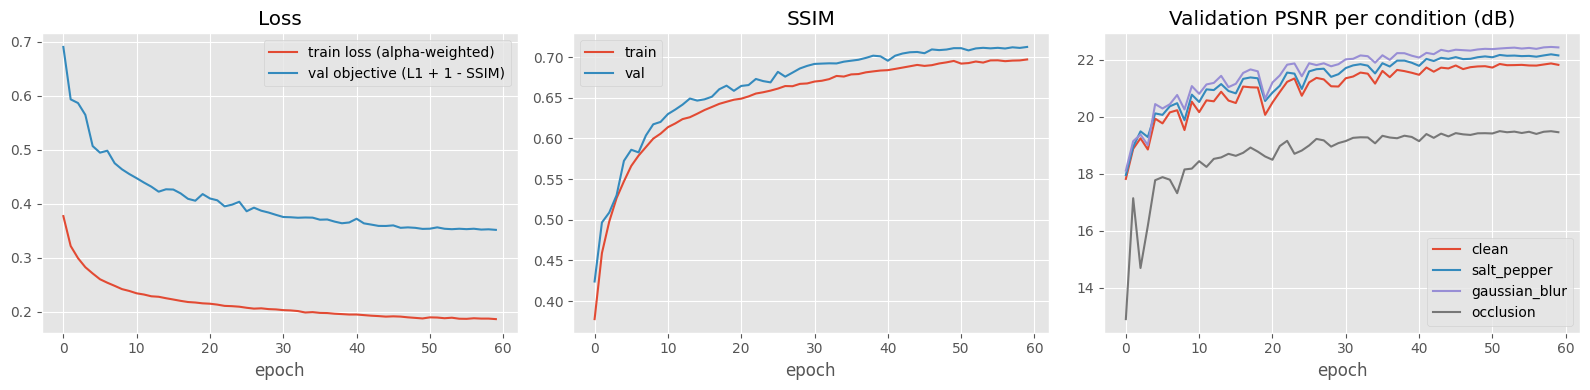
\includegraphics[width=\textwidth]{t1_curves.png}
\caption{Task 1 final training: loss, training and validation SSIM, and validation PSNR per condition.}
\label{fig:t1_curves}
\end{figure*}

\subsection{Results}
Table~\ref{tab:t1_results} reports the official test set (36,690 entries: 3,669 images under 10 conditions). Overall the model reaches PSNR 21.14\,dB, SSIM 0.704 and L1 0.066. Table~\ref{tab:t1_severity} separates the severity levels.

\begin{table}[t]
\centering
\caption{Task 1 test results by condition. ``Worse'' is the share of test entries where the output SSIM is below the input SSIM.}
\label{tab:t1_results}
\footnotesize
\setlength{\tabcolsep}{3.5pt}
\begin{tabular}{@{}lccccc@{}}
\toprule
Condition & In PSNR & Out PSNR & In SSIM & Out SSIM & Worse \\
\midrule
Clean & $\infty$ & 21.75 & 1.000 & 0.735 & 100\% \\
Salt-and-pepper & 16.38 & 21.79 & 0.382 & 0.731 & 7.1\% \\
Gaussian blur & 27.82 & 21.80 & 0.814 & 0.717 & 80.0\% \\
Occlusion & 13.64 & 19.63 & 0.713 & 0.654 & 66.6\% \\
\midrule
All & & 21.14 & & 0.704 & \\
\bottomrule
\end{tabular}
\end{table}

\begin{table}[t]
\centering
\caption{Task 1 test SSIM by corruption and severity.}
\label{tab:t1_severity}
\footnotesize
\setlength{\tabcolsep}{3.5pt}
\begin{tabular}{@{}llccc@{}}
\toprule
Corruption & Severity & In SSIM & Out SSIM & Out PSNR \\
\midrule
\multirow{3}{*}{Salt-and-pepper} & low ($p{=}0.03$) & 0.603 & 0.735 & 21.79 \\
 & medium ($p{=}0.08$) & 0.340 & 0.732 & 21.81 \\
 & high ($p{=}0.15$) & 0.204 & 0.727 & 21.77 \\
\midrule
\multirow{3}{*}{Gaussian blur} & low (3, 0.7) & 0.944 & 0.735 & 21.86 \\
 & medium (5, 1.5) & 0.806 & 0.725 & 21.91 \\
 & high (7, 2.5) & 0.692 & 0.690 & 21.63 \\
\midrule
\multirow{3}{*}{Occlusion} & low (10\%) & 0.862 & 0.698 & 20.67 \\
 & medium (20\%) & 0.731 & 0.661 & 19.72 \\
 & high (35\%) & 0.546 & 0.602 & 18.51 \\
\bottomrule
\end{tabular}
\end{table}

The most important observation is that output quality is almost independent of the input. Salt-and-pepper outputs reach SSIM 0.735, 0.732 and 0.727 whether the input SSIM was 0.60 or 0.20, and clean, noisy and blurred inputs all end near SSIM 0.73 and PSNR 21.8\,dB. The output is therefore limited by the 4,096-value bottleneck, not by the corruption. The consequences differ by corruption. Salt-and-pepper noise is removed almost completely (SSIM +0.35, worse in only 7.1\% of cases), because isolated extreme pixels carry little information and do not survive compression. Mild corruptions are made worse: a clean image loses 0.26 SSIM, low blur loses 0.21, and 80\% of blurred inputs leave the model with lower SSIM than they entered. Occlusion is the hardest condition (SSIM 0.654), because the model must invent content for up to 35\% of the image. Only at the highest occlusion level does the output beat the input SSIM.

Fig.~\ref{fig:t1_examples} shows twelve representative test entries (closest to the median SSIM of each condition and severity). Two systematic effects are visible beyond the scores. Fine texture such as fur is smoothed away, and colours are strongly desaturated: the red collar in the fourth row loses most of its colour. Both are consequences of compression, since the code keeps coarse shape and luminance better than texture and chroma. The absolute error maps confirm this, with errors concentrated on edges, texture and saturated colours.

\begin{figure*}[t]
\centering
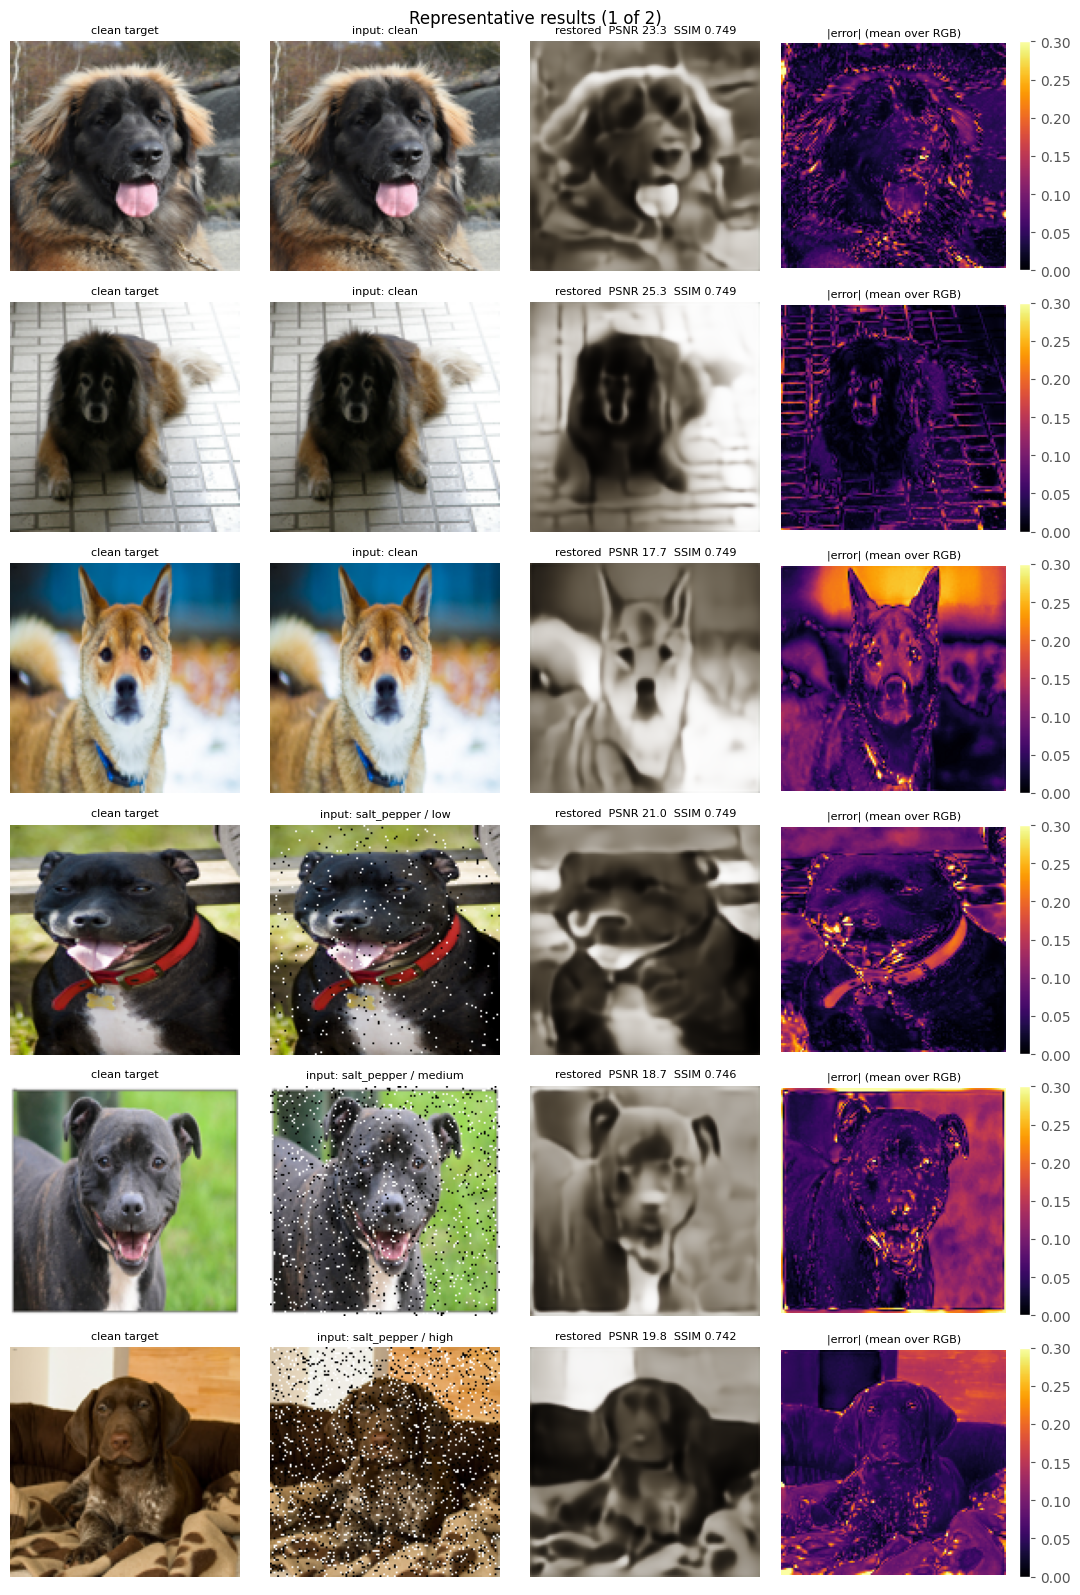
\includegraphics[width=0.48\textwidth]{t1_rep_a.png}\hfill
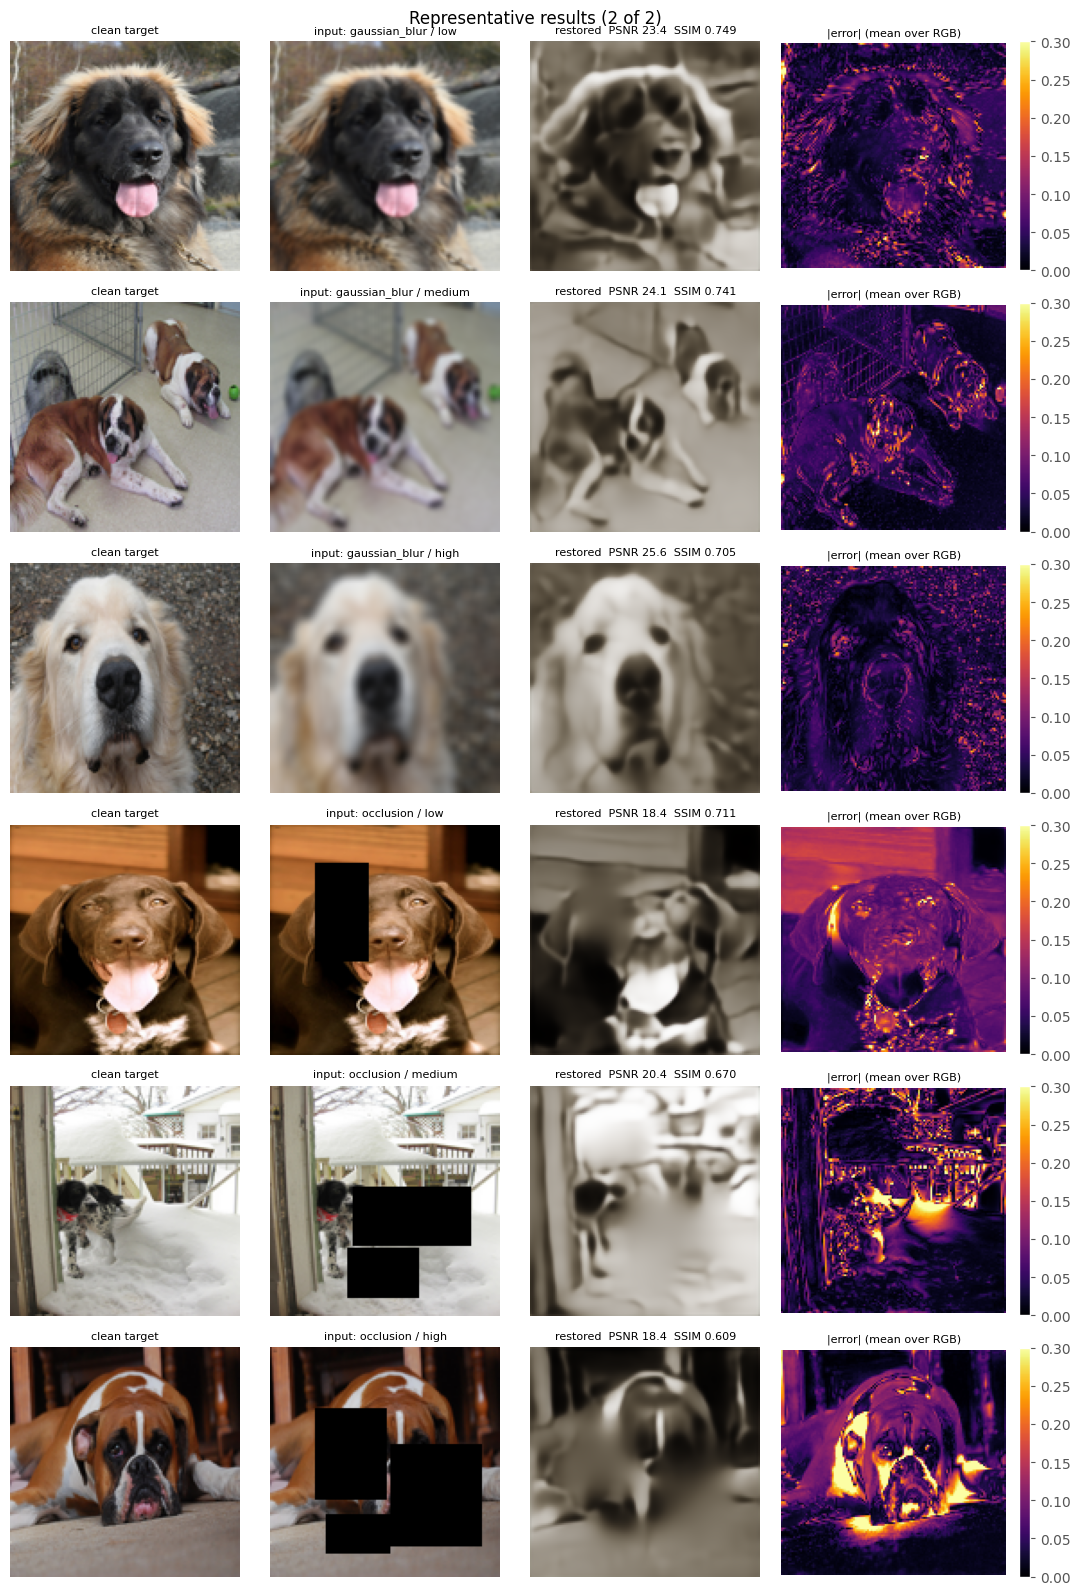
\includegraphics[width=0.48\textwidth]{t1_rep_b.png}
\caption{Task 1: twelve representative test results (clean target, model input, restoration, absolute error map). Left: clean and salt-and-pepper; right: Gaussian blur and occlusion, at each severity.}
\label{fig:t1_examples}
\end{figure*}

\textbf{Failure cases.} Fig.~\ref{fig:t1_fail} shows the lowest-SSIM entry for each condition. Three of the four failures are the same photograph: a dog in a meadow of flowers and grass. It fails as a clean image (SSIM 0.366), with salt-and-pepper noise (0.356) and with blur (0.296), so the failure is caused by image content rather than by the corruption. Dense high-frequency texture cannot be encoded in the latent code, and the decoder produces a smooth, colourless pattern. The fourth failure is a cat on a black background with heavy occlusion (SSIM 0.243). The model fills the occluded region and much of the dark background with light grey, the brightness of an average training image, so almost the whole background becomes error. Both failures show that a single compressed code learns a generic image prior that suits typical pet photographs but not unusual texture or lighting.

\begin{figure}[t]
\centering
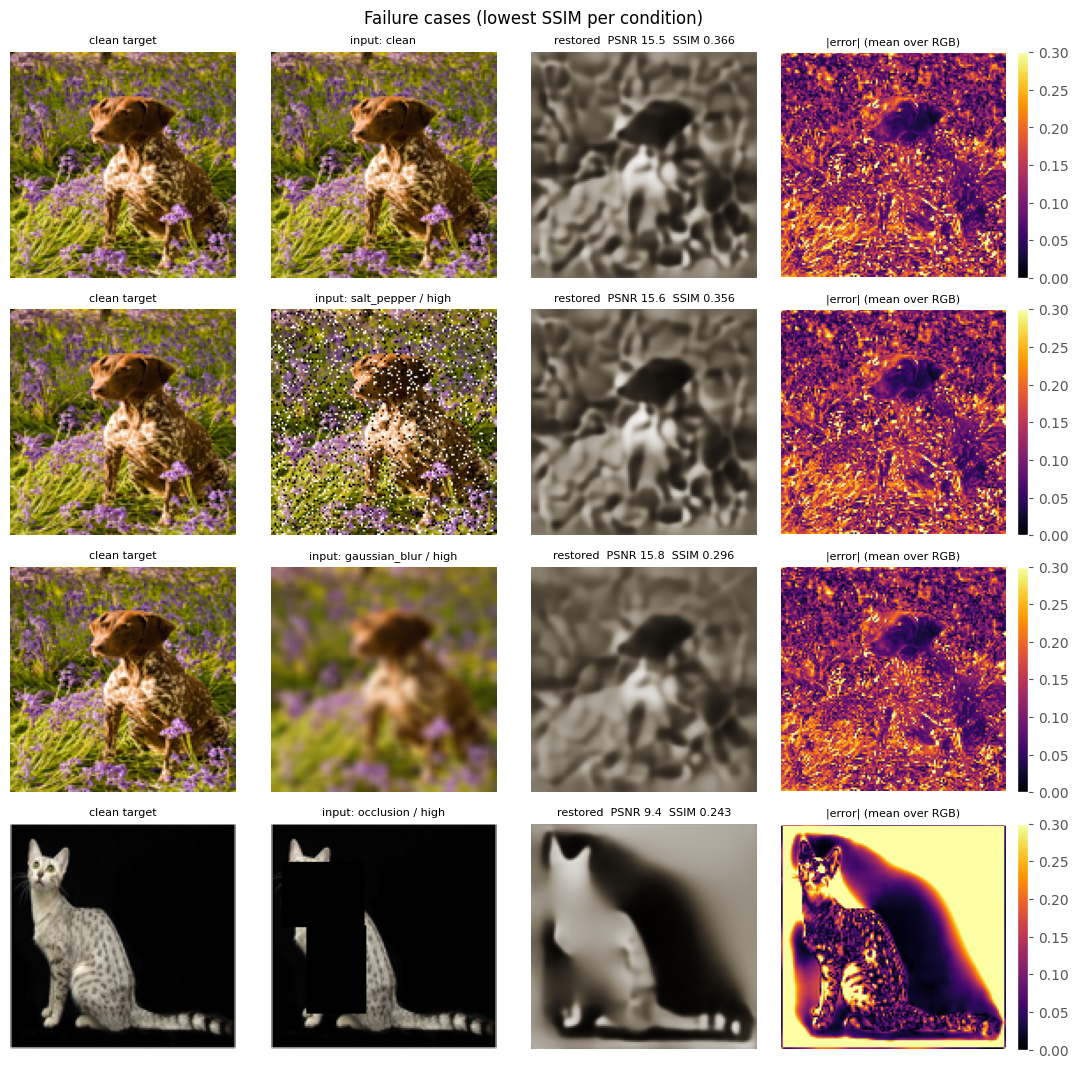
\includegraphics[width=\linewidth]{t1_fail.png}
\caption{Task 1 failure cases: lowest test SSIM per condition.}
\label{fig:t1_fail}
\end{figure}

\subsection{ONNX export}
The final model was exported to ONNX (opset 17, dynamic batch size; input \texttt{input}, output \texttt{output}, RGB in $[0,1]$). On 80 test entries covering every condition and severity, the maximum absolute difference to PyTorch was $7.2\times10^{-7}$. Single-image CPU latency on Colab was 110.8\,ms with ONNX Runtime against 140.3\,ms in PyTorch.

% =====================================================================
\section{Task 2: Corruption Classification and Hard-Routed Specialists}

\subsection{System overview}
Fig.~\ref{fig:t2_arch} shows the hard-routing system. A convolutional classifier predicts one of four classes; an argmax selects one branch. A clean prediction returns the input unchanged (identity bypass, no expert is run), and each corruption class sends the image to its own specialist autoencoder.

\begin{figure}[t]
\centering
\resizebox{\linewidth}{!}{%
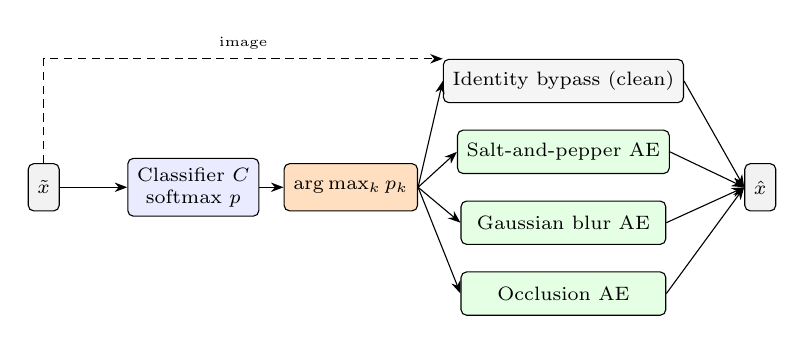
\begin{tikzpicture}[font=\scriptsize, >={Stealth[length=1.6mm]},
  box/.style={draw, rounded corners=2pt, align=center, minimum height=0.6cm},
  exp/.style={draw, rounded corners=2pt, align=center, fill=green!10, minimum width=2.6cm, minimum height=0.55cm}]
\node[box, fill=gray!10] (x) at (0,0) {$\tilde{x}$};
\node[box, fill=blue!8] (clf) at (1.9,0) {Classifier $C$\\softmax $p$};
\node[box, fill=orange!25] (am) at (3.9,0) {$\arg\max_k p_k$};
\node[exp, fill=gray!8] (b0) at (6.6,1.35) {Identity bypass (clean)};
\node[exp] (b1) at (6.6,0.45) {Salt-and-pepper AE};
\node[exp] (b2) at (6.6,-0.45) {Gaussian blur AE};
\node[exp] (b3) at (6.6,-1.35) {Occlusion AE};
\node[box, fill=gray!10] (y) at (9.1,0) {$\hat{x}$};
\draw[->] (x) -- (clf); \draw[->] (clf) -- (am);
\foreach \b in {b0,b1,b2,b3}{ \draw[->] (am.east) -- (\b.west); \draw[->] (\b.east) -- (y.west); }
\draw[->, densely dashed] (x.north) |- node[pos=0.75, above]{\tiny image} (b0.north west);
\end{tikzpicture}}
\caption{Task 2 hard routing: the classifier's most probable class selects exactly one branch. Only the selected specialist is run.}
\label{fig:t2_arch}
\end{figure}

\subsection{Corruption classifier}
The classifier has four stages of two 3$\times$3 convolutions (BatchNorm, ReLU), with max pooling between stages. The first stage runs at full resolution before any pooling, so isolated noise pixels and the edge sharpness that blur removes are still visible to it. Global average and global max pooling are concatenated, because a black occlusion box or a single noise pixel is a local, extreme response that average pooling alone would dilute; dropout and a linear layer then give four logits. Training labels come from the runtime corruption pipeline. A balanced batch sampler gives every batch exactly one quarter of each class while the severity is still sampled freshly (Fig.~\ref{fig:t2_batch}). The loss is multiclass cross-entropy, optimised with AdamW, cosine learning-rate decay and mixed precision; model selection uses validation macro-F1.

\begin{figure}[t]
\centering
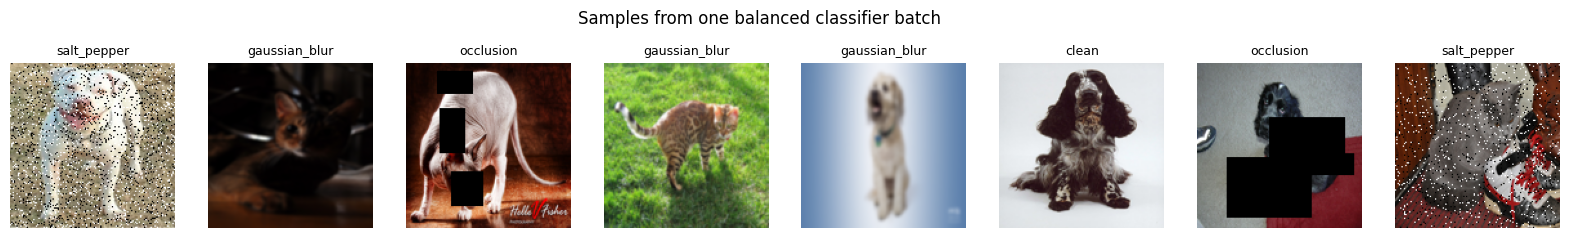
\includegraphics[width=\linewidth]{t2_balanced_batch.png}
\caption{Eight images from one balanced classifier batch: each of the four classes appears equally often, with freshly sampled severities.}
\label{fig:t2_batch}
\end{figure}

Optuna searched the learning rate, batch size, channel configuration, dropout and weight decay (Table~\ref{tab:t2_clf_optuna}) with 25 trials of 8 epochs; 11 completed and 14 were pruned. The task turned out to be easy: every completed trial reached a validation macro-F1 of at least 0.9946, and the best (trial 22) reached 1.000 on the 736 validation images. With differences of only one to four validation images between trials, the search could not separate configurations reliably, and the fANOVA importance (0.78 for dropout) should not be over-interpreted. The selected network is the smallest channel configuration (16, 32, 64, 128) with 295,028 parameters. The final classifier was trained for up to 40 epochs with patience 8; it stopped after epoch 25, and its best epoch was 17 (validation accuracy and macro-F1 0.9986, Fig.~\ref{fig:t2_clf_curves}). The validation spike at epoch 5 is a transient instability early in training that recovered by the next epoch.

\begin{table}[t]
\centering
\caption{Task 2 classifier: Optuna search space and selected values.}
\label{tab:t2_clf_optuna}
\footnotesize
\begin{tabular}{@{}lll@{}}
\toprule
Hyperparameter & Search range & Selected \\
\midrule
Learning rate & log-uniform $[10^{-4}, 3\times10^{-3}]$ & $2.94\times10^{-4}$ \\
Batch size & $\{32, 64, 128\}$ & 32 \\
Channels & 4 configurations\textsuperscript{a} & small \\
Dropout & uniform $[0, 0.5]$ & 0.113 \\
Weight decay & log-uniform $[10^{-6}, 10^{-2}]$ & $1.17\times10^{-5}$ \\
\bottomrule
\end{tabular}\\[2pt]
\parbox{0.95\linewidth}{\scriptsize \textsuperscript{a}small (16, 32, 64, 128), medium (32, 64, 128, 256), wide (48, 96, 192, 256), deep-narrow (32, 64, 96, 128).}
\end{table}

\begin{figure*}[t]
\centering
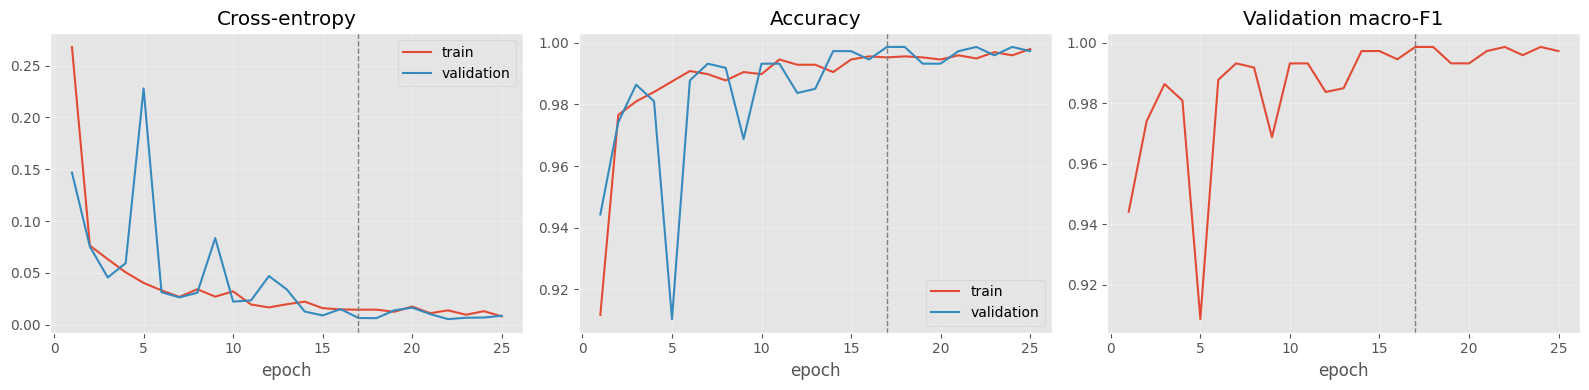
\includegraphics[width=\textwidth]{t2_clf_curves.png}
\caption{Task 2 classifier training: cross-entropy, accuracy and validation macro-F1. The dashed line marks the selected epoch.}
\label{fig:t2_clf_curves}
\end{figure*}

\textbf{Classifier results.} On the test set the classifier reaches an accuracy of 0.9986, macro-precision 0.9984, macro-recall 0.9970 and macro-F1 0.9977 (Table~\ref{tab:t2_clf_test}, Fig.~\ref{fig:t2_cm}). Salt-and-pepper noise is recognised perfectly. All of the remaining errors involve the clean class: 1.1\% of clean images are taken for occlusion (0.7\%) or blur (0.4\%), and a few low-severity blurred or occluded images are taken for clean. Fig.~\ref{fig:t2_clf_errors} shows the most confident mistakes. Clean photographs with large black regions (dark backgrounds, black cats, letterbox borders) are called occlusion, because they contain exactly the uniform black areas the occlusion class is defined by. Naturally soft or out-of-focus photographs are called blur. A blur of kernel 3 and $\sigma = 0.7$ is barely visible and was called clean. These errors are ambiguities in the data rather than arbitrary mistakes.

\begin{table}[t]
\centering
\caption{Task 2 classifier test results per class.}
\label{tab:t2_clf_test}
\footnotesize
\begin{tabular}{@{}lcccr@{}}
\toprule
Class & Precision & Recall & F1 & Support \\
\midrule
Clean & 0.9973 & 0.9888 & 0.9930 & 3,669 \\
Salt-and-pepper & 1.0000 & 1.0000 & 1.0000 & 11,007 \\
Gaussian blur & 0.9986 & 0.9995 & 0.9991 & 11,007 \\
Occlusion & 0.9976 & 0.9995 & 0.9985 & 11,007 \\
\midrule
Macro average & 0.9984 & 0.9970 & 0.9977 & 36,690 \\
\bottomrule
\end{tabular}
\end{table}

\begin{figure}[t]
\centering
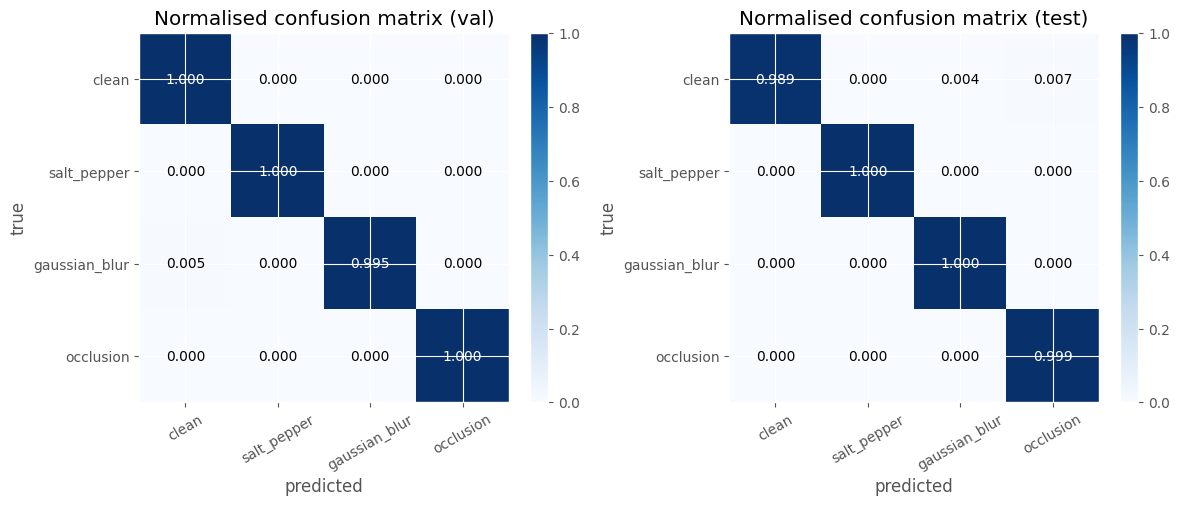
\includegraphics[width=\linewidth]{t2_confusion.png}
\caption{Row-normalised confusion matrices of the classifier on the validation set (left) and the test set (right).}
\label{fig:t2_cm}
\end{figure}

\begin{figure*}[t]
\centering
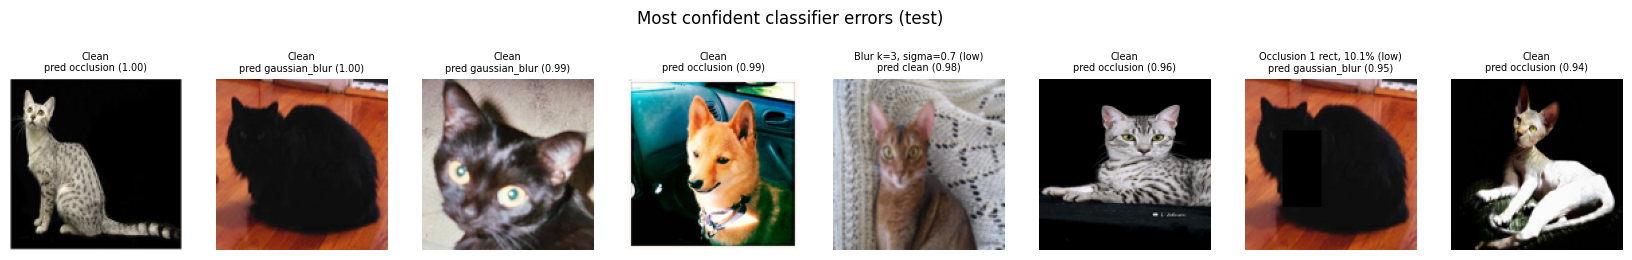
\includegraphics[width=\textwidth]{t2_clf_errors.png}
\caption{The most confident classifier errors on the test set (true class, predicted class and confidence).}
\label{fig:t2_clf_errors}
\end{figure*}

\subsection{Specialist autoencoders}
The three specialists use the Task 1 architecture with independently trained parameters, each trained only on its own corruption with the clean image as target and the loss of \eqref{eq:t1_loss}. To keep the search feasible, one shared Optuna study selected a common configuration, scored by the mean validation objective of all three specialists (15 trials of 8 epochs; 10 completed, 5 pruned). Dropout and the absence of skips were inherited from Task 1 so that the specialists differ from the universal model only in what they are trained on. The study selected learning rate $3.13\times10^{-4}$, batch size 16, $c = 48$, $L = 16$ and $\alpha = 0.526$ (objective 0.4550, trial 14; search ranges as in Table~\ref{tab:t1_optuna}). The fANOVA importance was 0.76 for $\alpha$ and 0.23 for the learning rate (Fig.~\ref{fig:t2_optuna}).

The specialists use a four-times smaller latent code than the universal model (1,024 values, 48:1 compression; 9,271,603 parameters each). A specialist only has to undo one kind of damage, so it needs less capacity for the same quality. Each specialist was trained for 60 epochs with patience 12 (Fig.~\ref{fig:t2_spec_curves}). The salt-and-pepper and blur specialists both reached validation SSIM 0.744, the occlusion specialist 0.643 (Table~\ref{tab:t2_spec}), and all three were still improving slightly at the end of training.

\begin{figure*}[t]
\centering
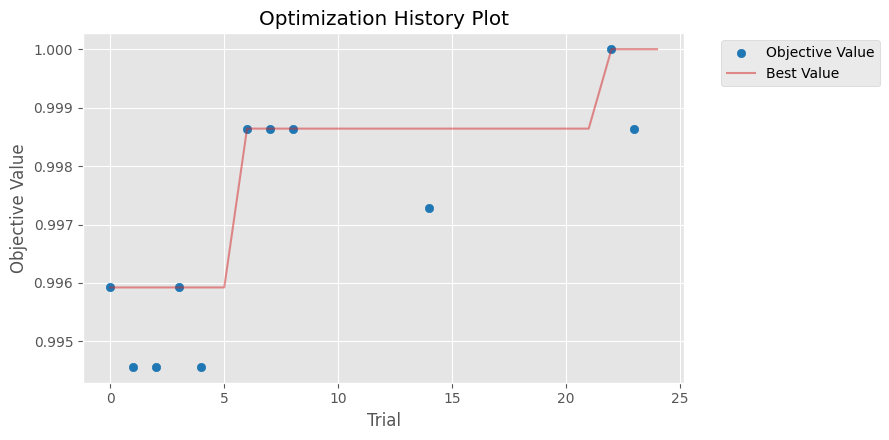
\includegraphics[width=0.32\textwidth]{t2_clf_optuna_history.png}\hfill
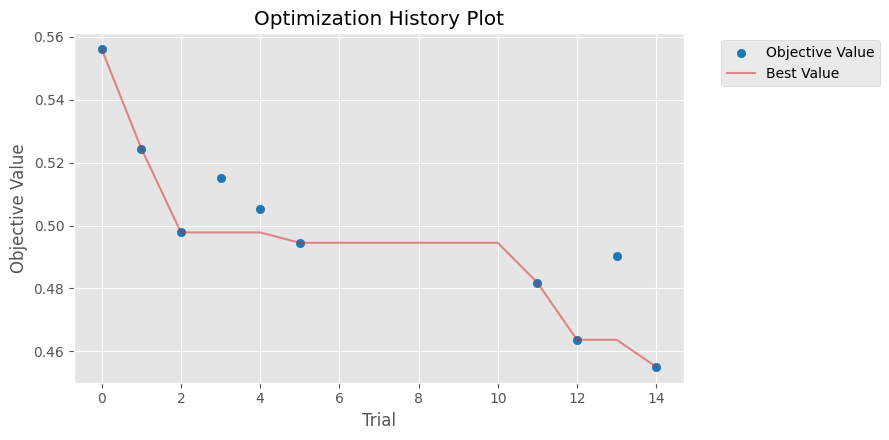
\includegraphics[width=0.32\textwidth]{t2_spec_optuna_history.png}\hfill
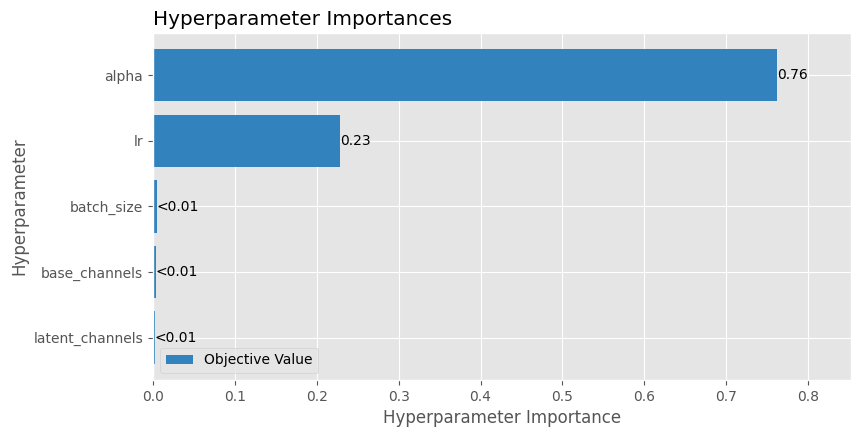
\includegraphics[width=0.32\textwidth]{t2_spec_optuna_importance.png}
\caption{Task 2 Optuna studies: classifier history (left, validation macro-F1, maximised), specialist history (centre, mean validation objective, minimised) and specialist hyperparameter importance (right).}
\label{fig:t2_optuna}
\end{figure*}

\begin{figure*}[t]
\centering
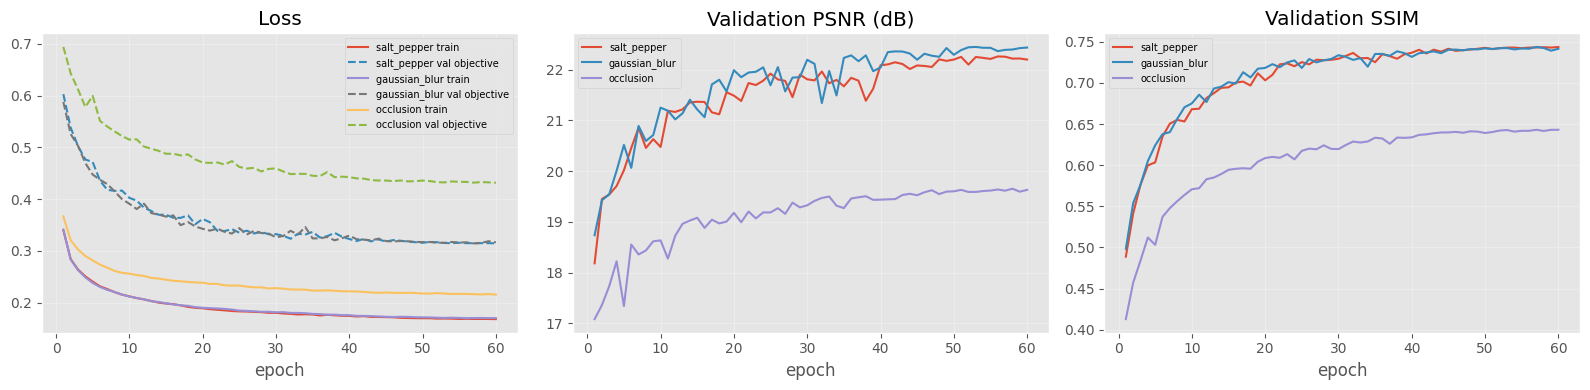
\includegraphics[width=\textwidth]{t2_spec_curves.png}
\caption{Training of the three specialists: training loss and validation objective, PSNR and SSIM.}
\label{fig:t2_spec_curves}
\end{figure*}

\begin{table}[t]
\centering
\caption{Specialists on their own validation corruption.}
\label{tab:t2_spec}
\footnotesize
\begin{tabular}{@{}lcccc@{}}
\toprule
Specialist & In PSNR & Out PSNR & In SSIM & Out SSIM \\
\midrule
Salt-and-pepper & 16.13 & 22.20 & 0.359 & 0.744 \\
Gaussian blur & 28.63 & 22.39 & 0.844 & 0.744 \\
Occlusion & 13.17 & 19.63 & 0.697 & 0.643 \\
\bottomrule
\end{tabular}
\end{table}

\subsection{Hard-routed restoration: oracle and predicted routing}
In oracle mode the true label from the test manifest selects the branch; in predicted mode the classifier selects it. Table~\ref{tab:t2_routing} compares both, and Table~\ref{tab:t2_vs_t1} compares them with the Task 1 universal model on exactly the same test entries.

\begin{table}[t]
\centering
\caption{Task 2 on the test set: routing accuracy and SSIM with oracle and predicted routing.}
\label{tab:t2_routing}
\footnotesize
\setlength{\tabcolsep}{4pt}
\begin{tabular}{@{}lccccc@{}}
\toprule
Condition & Routing acc. & In SSIM & Oracle & Predicted & Pred. PSNR \\
\midrule
Clean & 0.9888 & 1.000 & 1.000 & 0.997 & n/a \\
Salt-and-pepper & 1.0000 & 0.382 & 0.736 & 0.736 & 21.85 \\
Gaussian blur & 0.9995 & 0.814 & 0.727 & 0.727 & 21.81 \\
Occlusion & 0.9995 & 0.713 & 0.656 & 0.656 & 19.77 \\
\midrule
All corrupted & 0.9997 & 0.636 & 0.706 & 0.706 & 21.14 \\
\bottomrule
\end{tabular}
\end{table}

\begin{table}[t]
\centering
\caption{Test SSIM of the Task 1 universal model and Task 2 hard routing (predicted) on the same entries.}
\label{tab:t2_vs_t1}
\footnotesize
\begin{tabular}{@{}lccc@{}}
\toprule
Condition & Task 1 universal & Task 2 predicted & Difference \\
\midrule
Clean & 0.735 & 0.997 & $+0.262$ \\
Salt-and-pepper & 0.731 & 0.736 & $+0.005$ \\
Gaussian blur & 0.717 & 0.727 & $+0.010$ \\
Occlusion & 0.654 & 0.656 & $+0.002$ \\
\midrule
All 36,690 entries & 0.704 & 0.735 & $+0.031$ \\
\bottomrule
\end{tabular}
\end{table}

Because the classifier is almost perfect, predicted routing is practically identical to oracle routing: across all corrupted entries the SSIM lost to routing errors is below 0.001. Almost all of the gain over Task 1 comes from the identity bypass. Clean images keep SSIM 0.997 instead of 0.735, which lifts the overall test SSIM from 0.704 to 0.735. For corrupted images the specialists are only slightly better than the universal model (+0.002 to +0.010 SSIM), with the largest gain for high blur (0.714 against 0.690). Both systems share the same limitation: the specialists also produce outputs near SSIM 0.73 whatever the input, and for low blur they still degrade the image (0.944 input against 0.735 output). Specialisation therefore lets a smaller code do the same job, but it does not raise the quality ceiling set by the bottleneck. Fig.~\ref{fig:t2_rep} shows representative hard-routed results. The identity bypass returns clean images untouched, and the specialist outputs show the same smoothing and desaturation as Task 1.

\begin{figure*}[t]
\centering
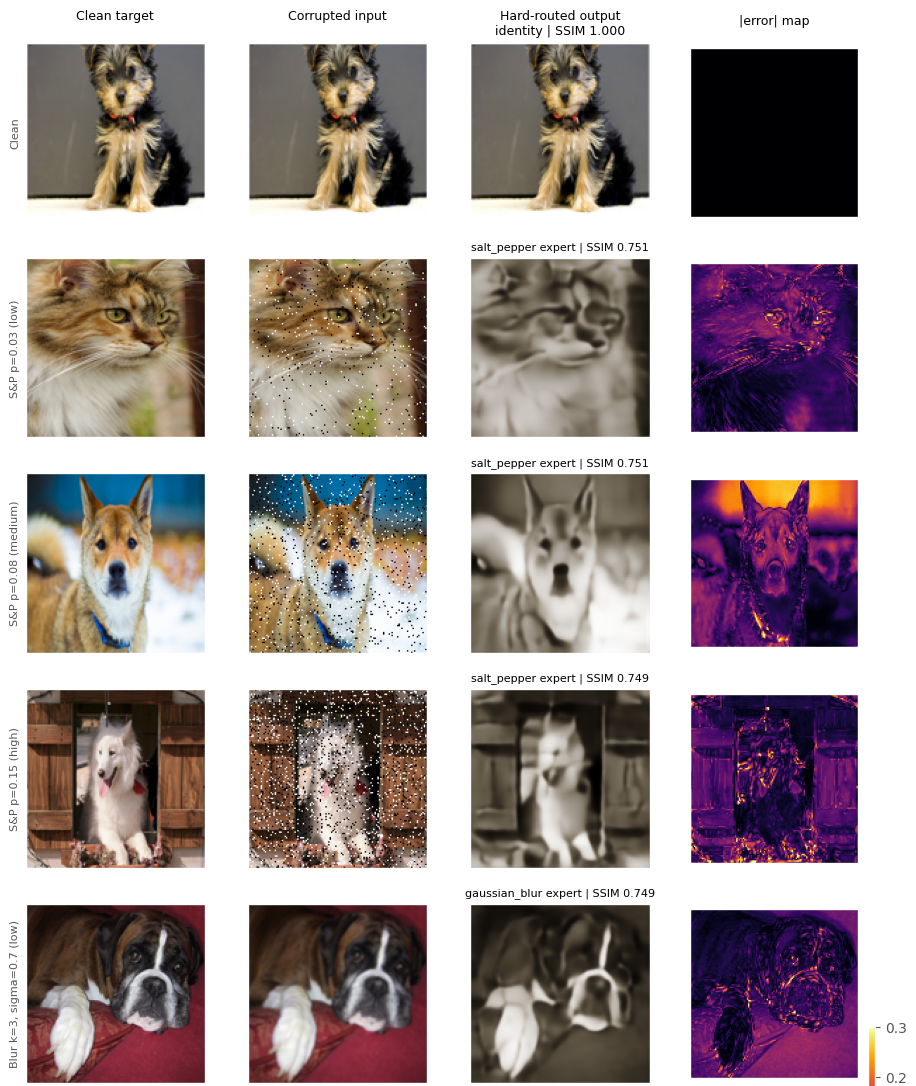
\includegraphics[width=0.48\textwidth]{t2_routing_rep_a.png}\hfill
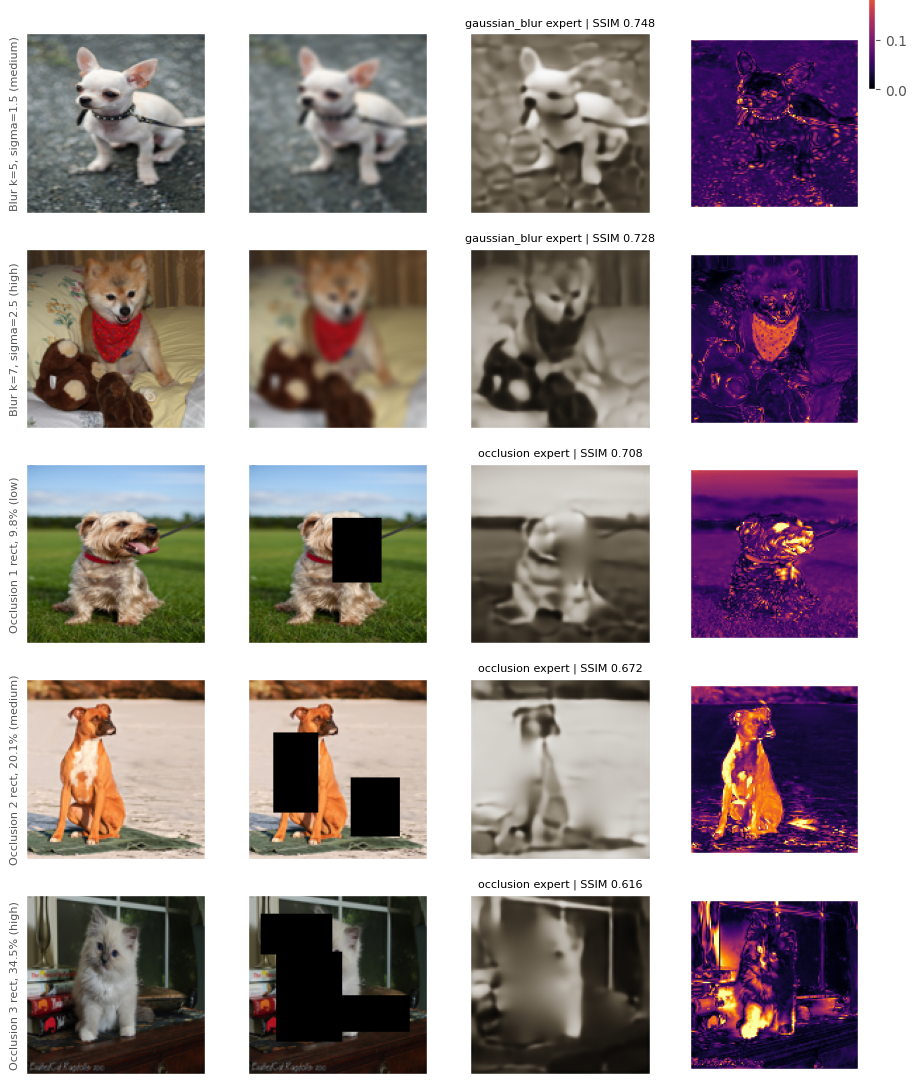
\includegraphics[width=0.48\textwidth]{t2_routing_rep_b.png}
\caption{Representative Task 2 results with predicted routing: clean target, model input, hard-routed output with the selected branch and SSIM, and absolute error map, for every condition and severity.}
\label{fig:t2_rep}
\end{figure*}

\textbf{Failures caused by classifier errors.} Only 52 of the 36,690 test entries (0.14\%) were misrouted (Table~\ref{tab:t2_misrouted}), and none of them was harmless: every routing error changed SSIM by at least 0.01. The costly errors are clean images sent to a specialist. A clean image sent to the occlusion or blur expert loses on average 0.27 or 0.22 SSIM, because a specialist always reconstructs through its bottleneck (Fig.~\ref{fig:t2_failures}). The worst cases are again photographs with black borders or dark backgrounds, and soft, low-contrast scenes. The reverse error has the opposite effect. When a low-severity blurred or occluded image was taken for clean, the identity bypass returned the mildly damaged input, which scored 0.28 and 0.12 SSIM \emph{higher} than the correct specialist would have achieved. This confirms the observation of Task 1: for light corruption, not restoring is better than restoring through the bottleneck, and a system that can weigh the identity branch against the experts could exploit this, which motivates the soft routing of Task 3.

\begin{table}[t]
\centering
\caption{Misrouted test entries by true and predicted class. SSIM lost is oracle minus predicted (negative values mean the routing error helped).}
\label{tab:t2_misrouted}
\footnotesize
\begin{tabular}{@{}llrcc@{}}
\toprule
True & Predicted & $n$ & Mean confidence & SSIM lost \\
\midrule
Clean & Gaussian blur & 14 & 0.764 & 0.221 \\
Clean & Occlusion & 27 & 0.753 & 0.265 \\
Gaussian blur & Clean & 5 & 0.748 & $-0.284$ \\
Occlusion & Clean & 5 & 0.733 & $-0.115$ \\
Occlusion & Gaussian blur & 1 & 0.950 & 0.106 \\
\bottomrule
\end{tabular}
\end{table}

\begin{figure}[t]
\centering
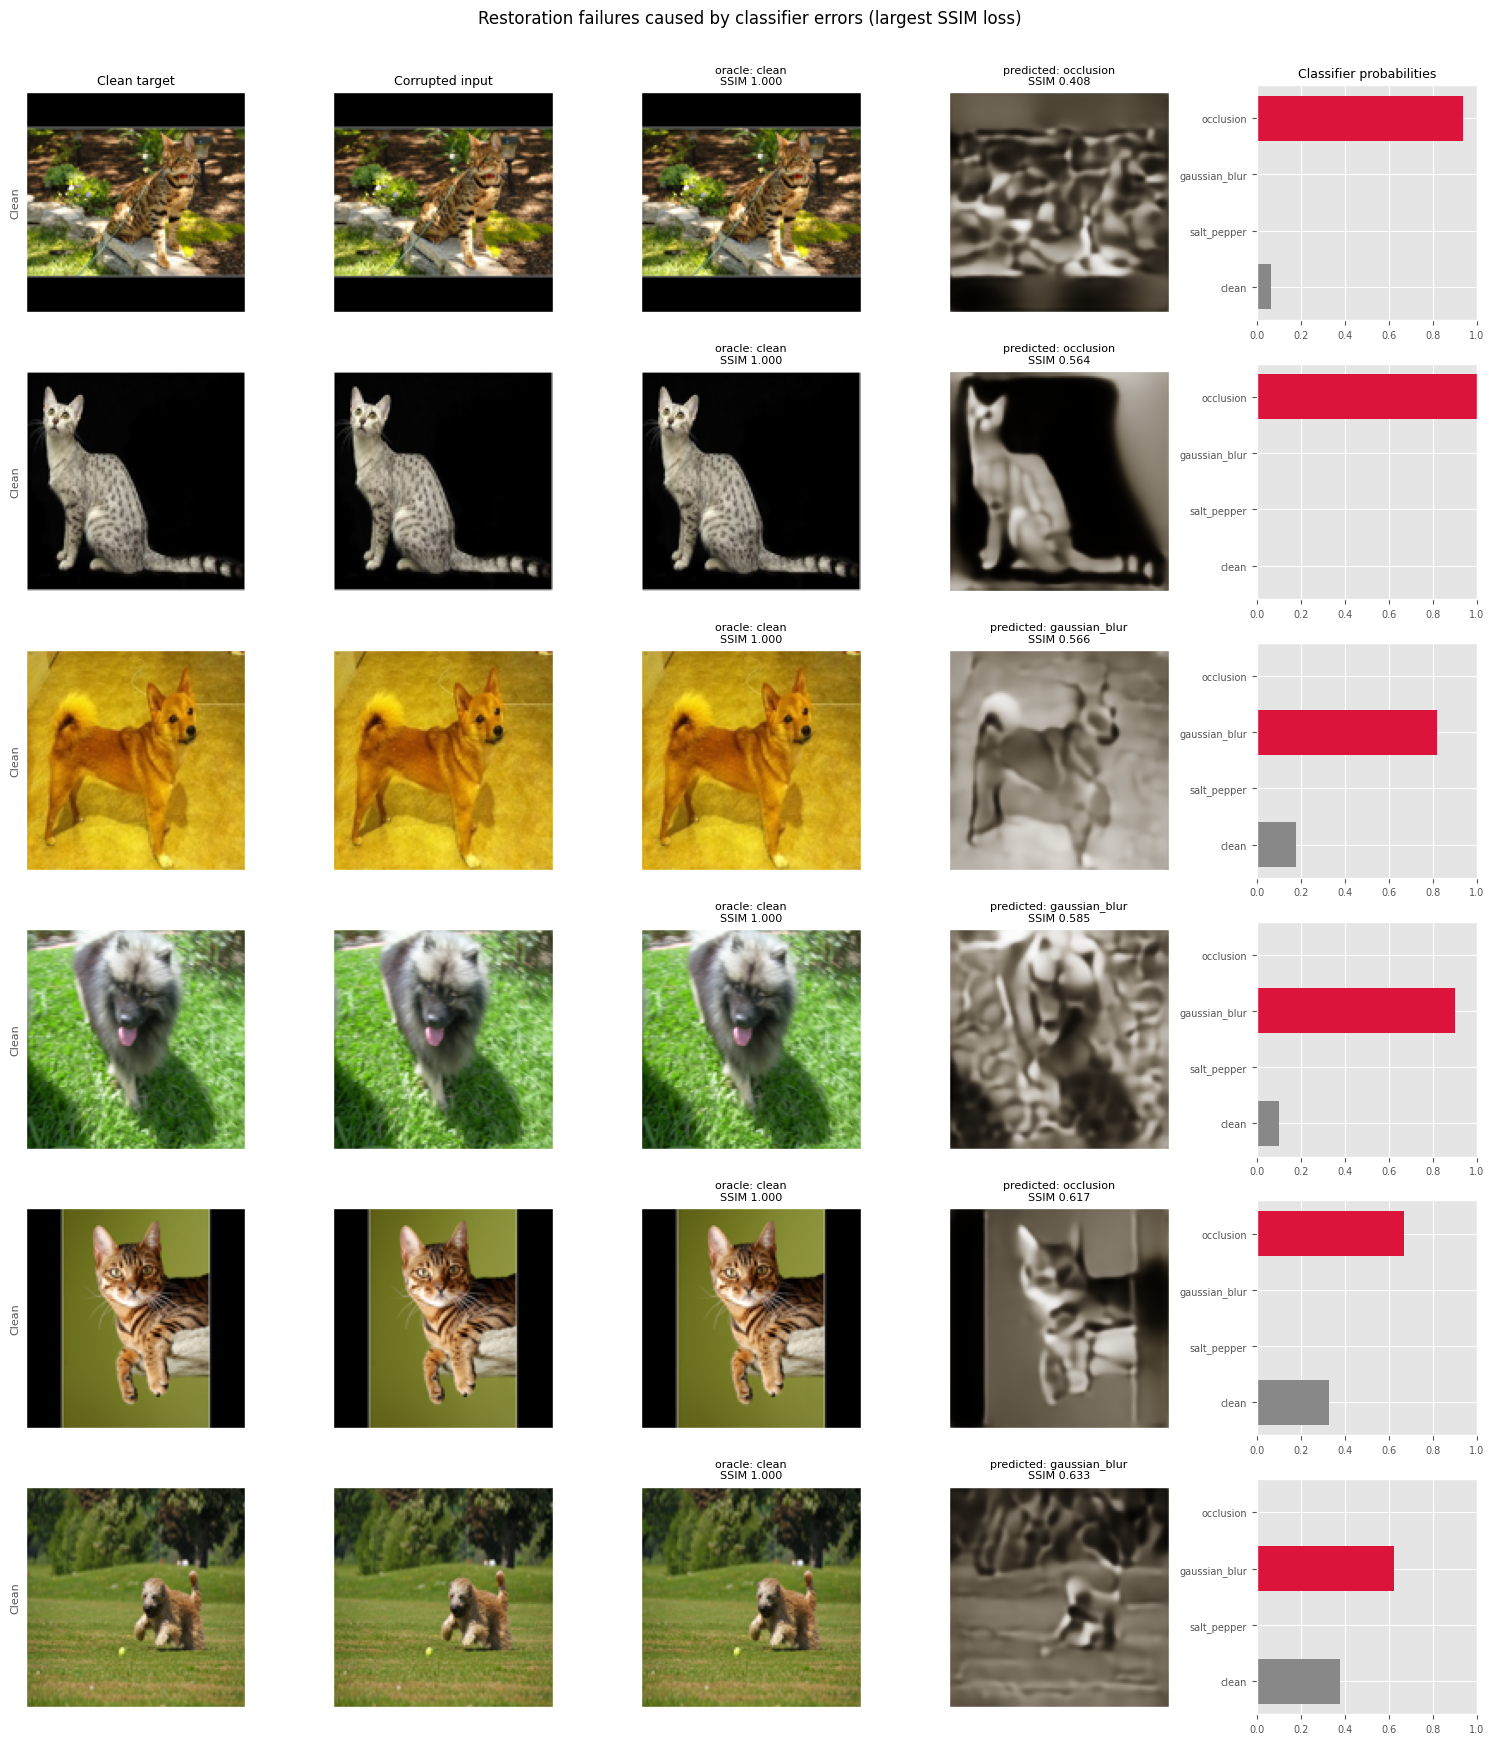
\includegraphics[width=\linewidth]{t2_routing_failures.png}
\caption{Restoration failures caused by classifier errors: clean images routed to a specialist, with oracle and predicted outputs and the classifier probabilities.}
\label{fig:t2_failures}
\end{figure}

\subsection{ONNX export}
The classifier (wrapped to output both logits and probabilities) and the three specialists were exported to ONNX (opset 17, dynamic batch size). On 80 test entries the classifier's probabilities differed from PyTorch by at most $1.5\times10^{-7}$ with identical predicted classes, and the specialists by at most $0.9\times10^{-6}$ to $2.1\times10^{-6}$. On the Colab CPU the classifier takes 5.9\,ms per image and a specialist 110 to 134\,ms. The classifier adds only about 5\% to the cost of a restoration, and the identity bypass skips the expert entirely for clean images.

% =====================================================================
\section{Task 3: Jointly Trained Soft Mixture of Experts}

\subsection{Model}
The gating network $g$ is initialised from the Task 2 classifier (295,028 parameters) and outputs four logits. Routing weights are
\begin{equation}
w = \text{softmax}\bigl(g(\tilde{x}) / T\bigr), \quad w = [w_0, w_1, w_2, w_3],
\end{equation}
and the restored image is
\begin{equation}
\hat{x} = w_0 \tilde{x} + w_1 E_{\text{salt}}(\tilde{x}) + w_2 E_{\text{blur}}(\tilde{x}) + w_3 E_{\text{occ}}(\tilde{x}),
\end{equation}
where branch 0 is an identity branch and the three experts (27,814,809 parameters in total) are initialised from the Task 2 specialists. Unlike hard routing, every branch is evaluated for every image, and because the combination is differentiable the gate and experts can be trained jointly through the reconstruction error. Before training, the loaded components reproduced the Task 2 results on the validation set (classifier accuracy 0.9986; hard-routing SSIM 0.7831 predicted and 0.7826 oracle), which confirmed that they were loaded correctly.

\subsection{Loss}
\begin{equation}
\mathcal{L}_{\text{MoE}} = \lambda_1 \mathcal{L}_1 + \lambda_2 (1 - \text{SSIM}) + \lambda_3 \mathcal{L}_{\text{CE}} + \lambda_4 \mathcal{L}_{\text{balance}},
\end{equation}
with $\mathcal{L}_{\text{balance}} = \sum_{k=0}^{3} (\bar{w}_k - \tfrac{1}{4})^2$, where $\bar{w}_k$ is the mean weight of branch $k$ in a batch. A balanced batch sampler gives every batch exactly one quarter of each condition, so perfect routing gives $\bar{w}_k = 1/4$ and the balance term is zero at that solution; it only penalises collapse onto a subset of branches, in the spirit of load-balancing losses \cite{shazeer2017,fedus2022}. The cross-entropy term is applied to the raw gate logits, so it ties the gate to the corruption label while $T$ alone controls the sharpness of the routing. The reconstruction weighting is $\lambda_1 = a$, $\lambda_2 = 1 - a$.

\subsection{Training and hyperparameter optimisation}
Training starts with a warm-up in which the experts are frozen (no gradients and fixed BatchNorm statistics) and only the gate is trained (learning rate $3\times10^{-4}$), followed by joint fine-tuning of all components with a smaller learning rate. The batch size is 32. Optuna tuned the joint learning rate, $T$, $\lambda_3$, $\lambda_4$ and $a$ (Table~\ref{tab:t3_optuna}). Each trial ran one warm-up and four joint epochs and was scored on the validation objective $\text{L1} + (1-\text{SSIM})$. Trial 0 used the starting values suggested in the brief ($a = 0.8$, $\lambda_3 = 0.1$, $\lambda_4 = 0.01$, $T = 1$). Trials were pruned by the median rule, or when any branch received less than 5\% of the average weight on the balanced validation set (routing collapse).

\begin{table}[t]
\centering
\caption{Task 3 Optuna search space and the selected configuration (trial 13).}
\label{tab:t3_optuna}
\footnotesize
\begin{tabular}{@{}lll@{}}
\toprule
Hyperparameter & Search range & Selected \\
\midrule
Joint learning rate & log-uniform $[10^{-5}, 3\times10^{-4}]$ & $2.09\times10^{-4}$ \\
Temperature $T$ & log-uniform $[0.3, 3]$ & 0.607 \\
CE weight $\lambda_3$ & log-uniform $[0.01, 1]$ & 0.0115 \\
Balance weight $\lambda_4$ & log-uniform $[10^{-3}, 1]$ & 0.0378 \\
Reconstruction weight $a$ & uniform $[0.5, 0.95]$ & 0.703 \\
\midrule
Validation objective & & 0.2087 \\
\bottomrule
\end{tabular}
\end{table}

Twenty-one trials were recorded: 16 completed, 4 were pruned and 1 was interrupted by a session disconnect and never finished. The brief's starting values scored about 0.26, and the best trial reached 0.2087 (Fig.~\ref{fig:t3_optuna}). The fANOVA importance assigns 0.93 to the joint learning rate and almost nothing to the other parameters. The trial logs reveal a clear trade-off that the importance plot hides. Trials with a large CE weight or a high temperature (for example trial 10: $\lambda_3 = 0.29$, $T = 2.7$) kept the gate's argmax accuracy near 0.999 but reached only about 0.80 validation SSIM. Trials with $\lambda_3 \approx 0.01$ to $0.02$ let the identity branch take more than half of the weight, lowering argmax accuracy to about 0.6, and reached 0.83. The objective therefore rewarded a gate that stops behaving like a classifier and starts acting as a mixer. Trial 15 was pruned by the collapse rule after the blur branch fell to 4.8\% of the weight.

\begin{figure}[t]
\centering
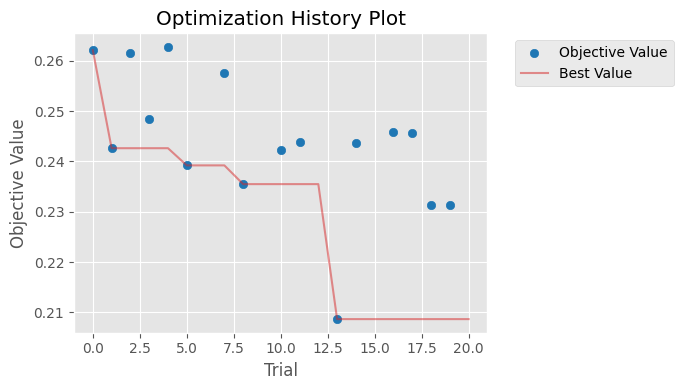
\includegraphics[width=0.95\linewidth]{t3_optuna_history.png}\\[2pt]
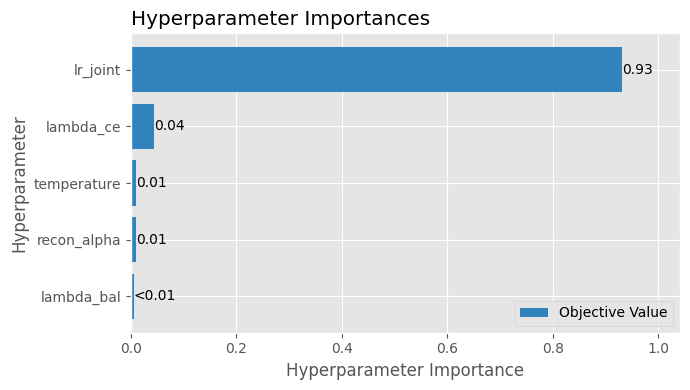
\includegraphics[width=0.95\linewidth]{t3_optuna_importance.png}
\caption{Task 3 Optuna study: objective per trial (top) and fANOVA importance (bottom).}
\label{fig:t3_optuna}
\end{figure}

The final model was trained with three warm-up epochs and up to 35 joint epochs with patience 8. It stopped after epoch 37; the best checkpoint is from epoch 29, with validation objective 0.1968 and validation SSIM 0.8394 (Fig.~\ref{fig:t3_curves}). Most of the improvement happened during warm-up, while the experts were still frozen. Validation SSIM rose from 0.783 (the hard-routing starting point) to 0.825 after three warm-up epochs, only because the gate learned to mix the identity branch with the experts. Joint fine-tuning then added another 0.015. Over the same period the share of weight on the identity branch grew from about 0.41 to 0.59 on the balanced validation set.

\begin{figure*}[t]
\centering
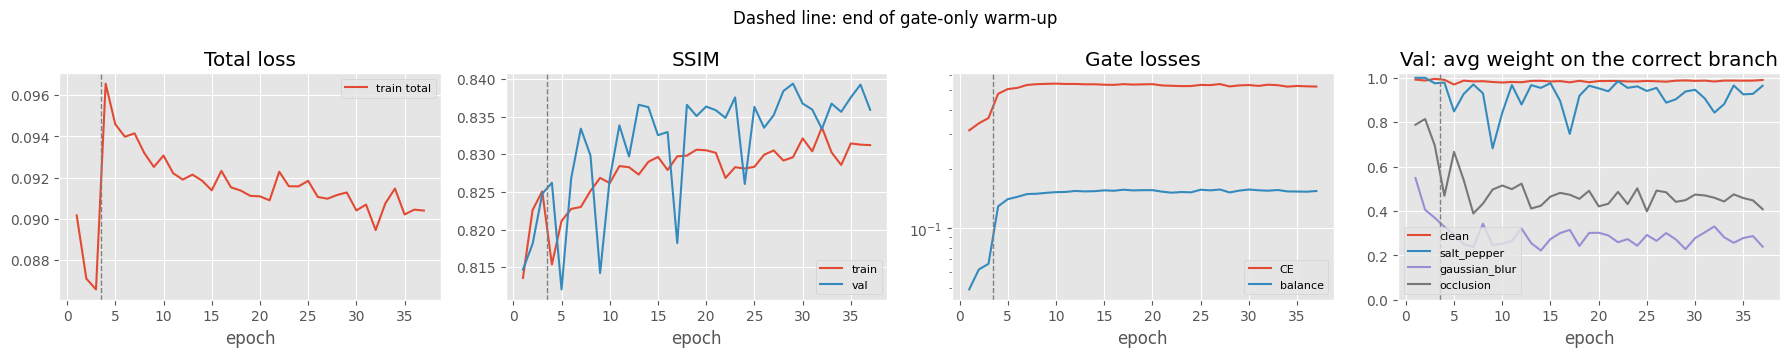
\includegraphics[width=\textwidth]{t3_curves.png}
\caption{Task 3 final training. The dashed line marks the end of the gate-only warm-up. Right: average validation weight on the correct branch for each true condition.}
\label{fig:t3_curves}
\end{figure*}

\subsection{Restoration quality}
On the validation manifest (736 images, 184 per condition, identical inputs for both systems), the soft mixture of experts reaches SSIM 0.839, against 0.783 for Task 2 hard routing with predicted labels and 0.783 with oracle labels: a gain of 0.056 from soft weighting alone. Since oracle routing is no better than predicted routing, the gain does not come from correcting classifier errors. It comes from blending.

\subsection{Routing behaviour}
Table~\ref{tab:t3_routing} and Fig.~\ref{fig:t3_heatmap} give the mean routing weight for every true corruption and severity on the test set, and Fig.~\ref{fig:t3_dist} shows the distributions. The gate learned three distinct behaviours:
\begin{itemize}
\item \textbf{Clean images} go almost entirely to the identity branch (0.987), as in Task 2.
\item \textbf{Salt-and-pepper noise} goes mainly to its expert, and more so as the noise increases (0.80, 0.95 and 0.98 for the three levels). Noise is the one corruption the expert removes far better than leaving the input alone.
\item \textbf{Blur and occlusion} are blends of the identity branch and the matching expert, and the weight moves towards the expert as severity increases. Identity receives 0.88, 0.74 and 0.63 for the three blur levels, and 0.70, 0.55 and 0.41 for the three occlusion levels.
\end{itemize}
This severity-dependent blending is exactly what the Task 1 and Task 2 results suggested. Every expert reconstructs through a bottleneck that limits output SSIM to about 0.73, so for mild damage the input itself is closer to the clean image than any reconstruction. The gate discovered this without being told.

\begin{table}[t]
\centering
\caption{Mean routing weight by true corruption and severity (test set).}
\label{tab:t3_routing}
\footnotesize
\setlength{\tabcolsep}{4pt}
\begin{tabular}{@{}llcccc@{}}
\toprule
True & Severity & Identity & S\&P exp. & Blur exp. & Occl. exp. \\
\midrule
Clean & & 0.987 & 0.000 & 0.002 & 0.011 \\
\midrule
\multirow{3}{*}{Salt-and-pepper} & low & 0.192 & 0.802 & 0.000 & 0.006 \\
 & medium & 0.053 & 0.946 & 0.000 & 0.001 \\
 & high & 0.023 & 0.977 & 0.000 & 0.000 \\
\midrule
\multirow{3}{*}{Gaussian blur} & low & 0.884 & 0.000 & 0.111 & 0.005 \\
 & medium & 0.739 & 0.000 & 0.256 & 0.004 \\
 & high & 0.627 & 0.000 & 0.368 & 0.004 \\
\midrule
\multirow{3}{*}{Occlusion} & low & 0.695 & 0.000 & 0.000 & 0.305 \\
 & medium & 0.555 & 0.000 & 0.000 & 0.445 \\
 & high & 0.413 & 0.000 & 0.000 & 0.587 \\
\bottomrule
\end{tabular}
\end{table}

\begin{figure}[t]
\centering
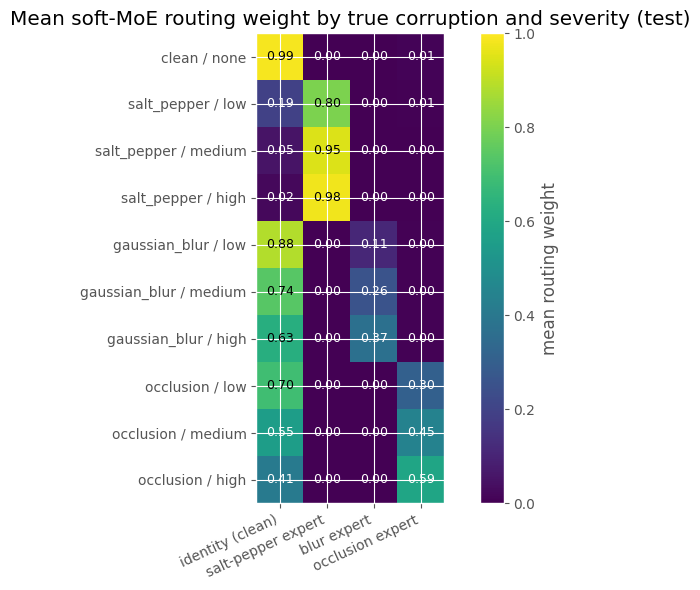
\includegraphics[width=0.92\linewidth]{t3_routing_heatmap.png}
\caption{Routing heatmap: mean weight of each branch for every true corruption and severity (test set).}
\label{fig:t3_heatmap}
\end{figure}

\begin{figure*}[t]
\centering
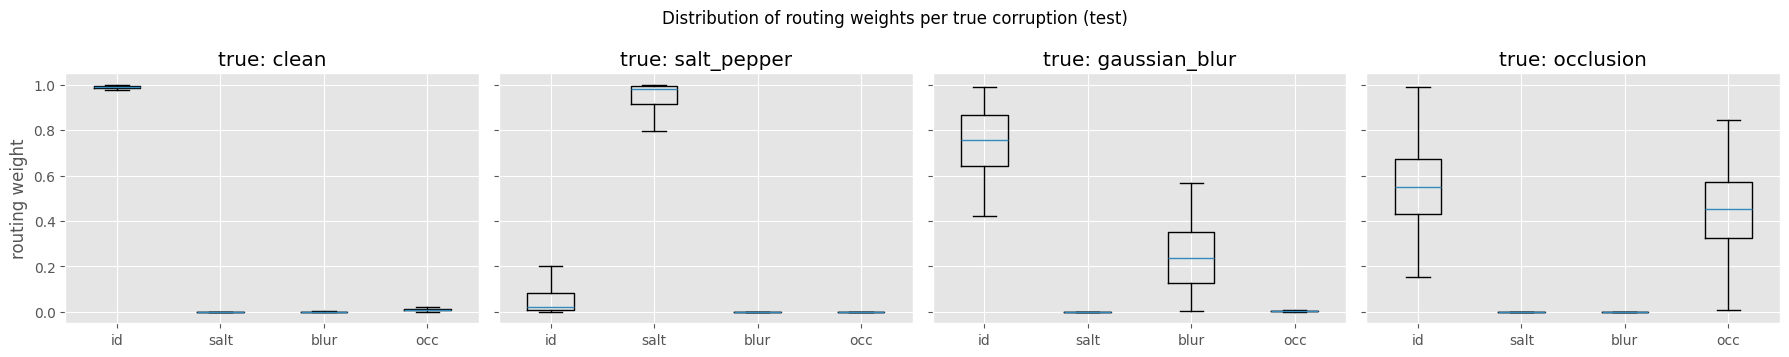
\includegraphics[width=\textwidth]{t3_routing_distributions.png}
\caption{Distribution of the four routing weights for each true corruption (test set).}
\label{fig:t3_dist}
\end{figure*}

\textbf{Inactive or dominant experts.} Table~\ref{tab:t3_usage} summarises how much each branch is used. No branch collapsed completely, but the experts are used very unevenly. The blur expert is nearly inactive as a decision-maker: its mean weight is 0.074 and it is the strongest branch for only 0.1\% of test images (its largest weight anywhere is 0.567), so blurred images are restored mostly by keeping the input. The identity branch is dominant: it receives a mean weight of 0.465 on inputs that are not clean, which the automatic check flags as dominance over unrelated inputs. The experts themselves stay specific: none receives more than 0.005 weight on corruptions other than its own. The behaviour follows from the selected loss weights. With $\lambda_3 = 0.0115$ the label constraint is weak, and the balance term only penalises averages over a batch, so it cannot stop a branch from being used as a partial blend for most images.

\begin{table}[t]
\centering
\caption{Branch usage on the test set.}
\label{tab:t3_usage}
\footnotesize
\setlength{\tabcolsep}{3.5pt}
\begin{tabular}{@{}lcccc@{}}
\toprule
Branch & Mean weight & Strongest for & Own type & Other types \\
\midrule
Identity & 0.517 & 59.3\% & 0.987 & 0.465 \\
Salt-and-pepper & 0.273 & 28.6\% & 0.908 & 0.000 \\
Gaussian blur & 0.074 & 0.1\% & 0.245 & 0.000 \\
Occlusion & 0.137 & 12.0\% & 0.446 & 0.005 \\
\bottomrule
\end{tabular}
\end{table}

\textbf{Dominant and distributed examples.} Fig.~\ref{fig:t3_examples} shows the test images with the lowest and highest routing entropy. When one branch dominates, the result is clean and predictable: a clean image passes through unchanged (SSIM 0.999) and medium salt-and-pepper noise goes entirely to its expert. The other two dominant cases show the limit of optimising SSIM. A lightly blurred image is left blurred (SSIM 0.811), and a lightly occluded image keeps its black box (SSIM 0.892), because the gate scores these as better than any reconstruction even though a person would prefer the box to be filled. Distributed weights produce visible ghosting. A 0.5/0.5 blend of input and occlusion expert gives semi-transparent grey boxes, and an identity-heavy blend for light noise leaves part of the noise in the output (SSIM 0.593). The last example is the dark-background cat that Task 2 misrouted to the occlusion expert (SSIM 0.564 there). Here the gate splits its weight evenly between identity and the occlusion expert, which halves the damage (SSIM 0.618) instead of committing to the wrong branch.

\begin{figure*}[t]
\centering
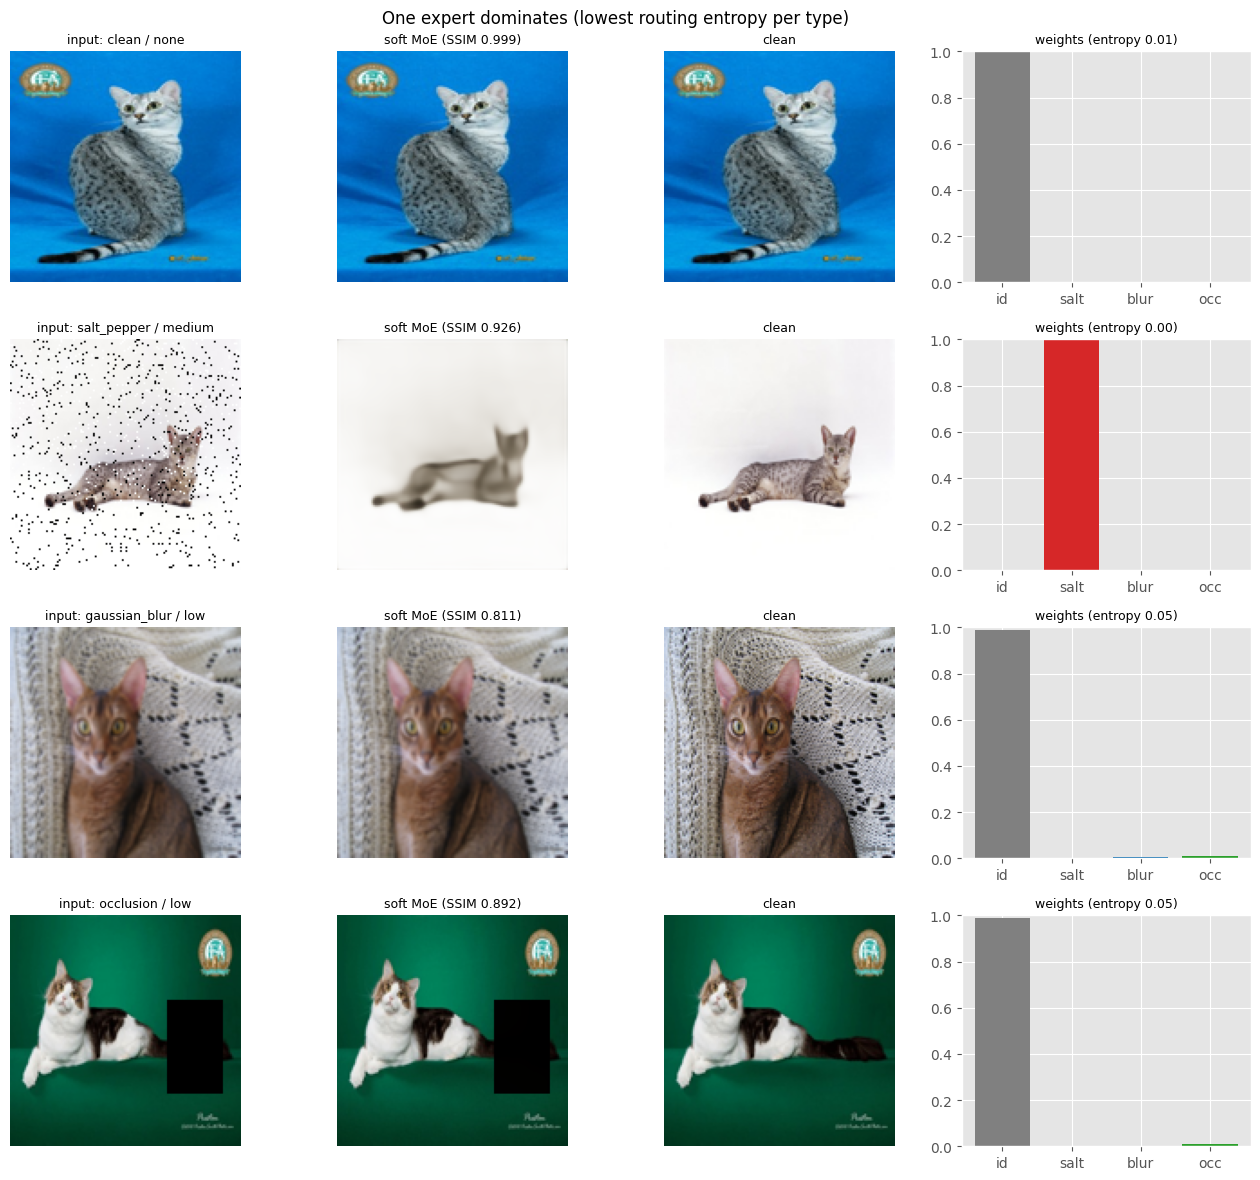
\includegraphics[width=0.49\textwidth]{t3_routing_dominant.png}\hfill
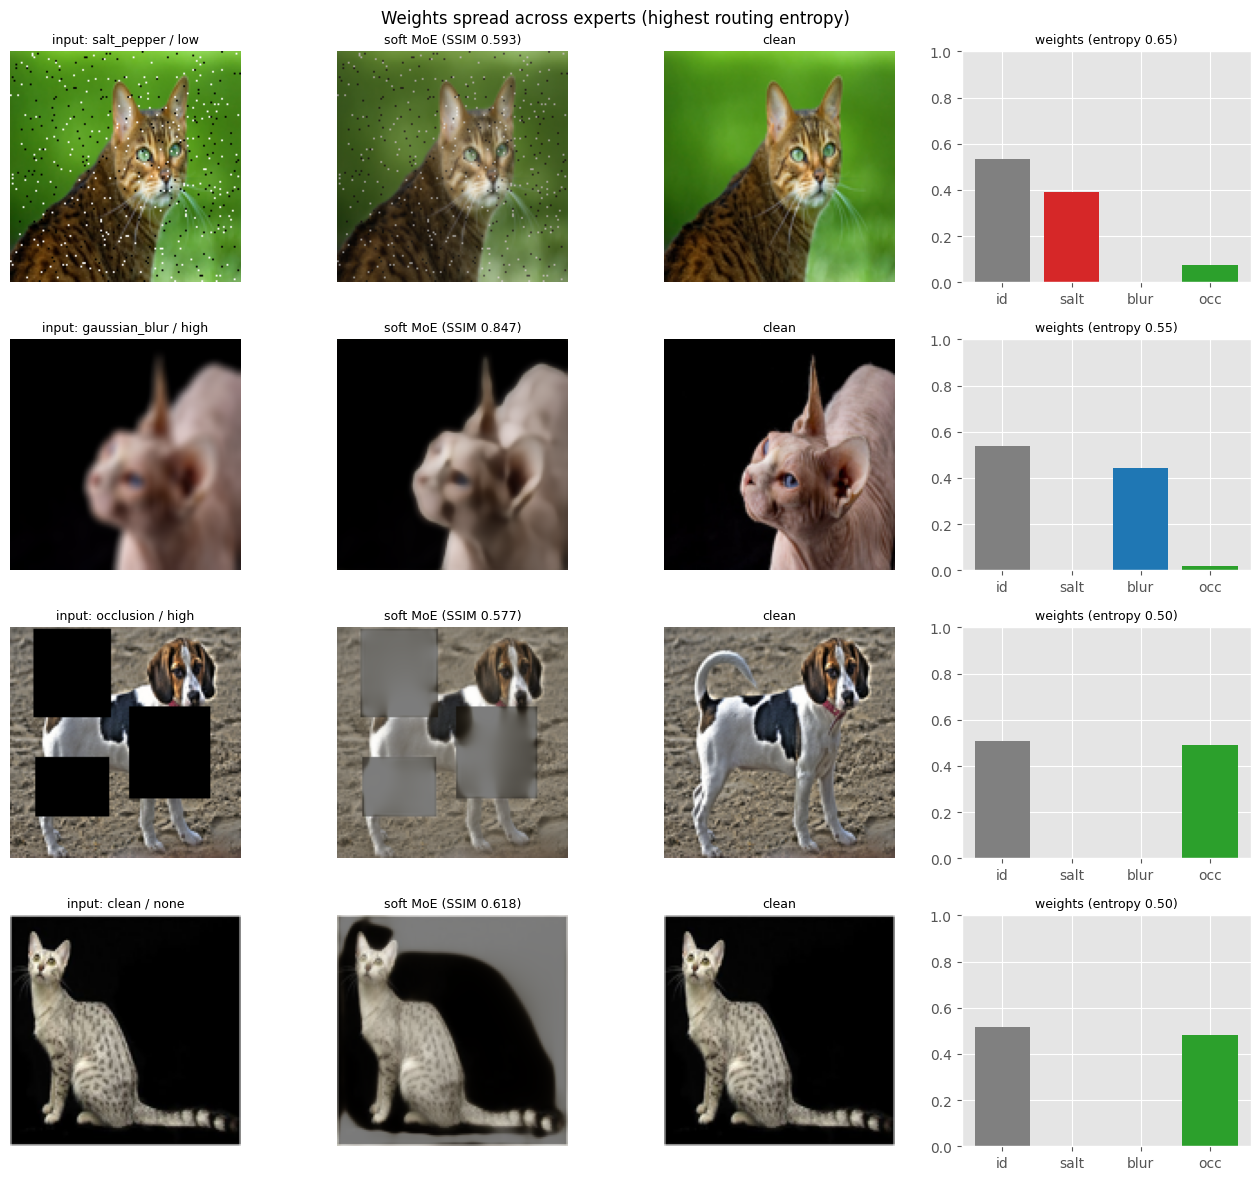
\includegraphics[width=0.49\textwidth]{t3_routing_distributed.png}
\caption{Soft MoE test examples with routing weights. Left: one branch dominates (lowest routing entropy per type). Right: weights spread across branches (highest entropy).}
\label{fig:t3_examples}
\end{figure*}

\textbf{Two corruptions in one image.} Hard routing can only choose one expert, so 300 test images were also corrupted twice at medium severity (Table~\ref{tab:t3_mixed}). For blur plus occlusion the gate blends identity (0.53) with the occlusion expert (0.47) and beats hard routing (0.644 against 0.632). For blur plus noise it sends almost everything to the noise expert (0.994), which also removes the blur, and matches hard routing. For noise plus occlusion it mixes identity (0.55) and the noise expert (0.44); the identity share keeps part of the noise, so soft routing is worse (0.390 against 0.435). The blur expert is never chosen for these combinations, which matches its low use in Table~\ref{tab:t3_usage}.

\begin{table}[t]
\centering
\caption{Images with two corruptions (300 test images per pair): SSIM and mean soft-MoE weights.}
\label{tab:t3_mixed}
\footnotesize
\setlength{\tabcolsep}{3pt}
\begin{tabular}{@{}lccccc@{}}
\toprule
Pair & Input & Hard & Soft & $w_{\text{id}}$ & Main expert \\
\midrule
Blur + occlusion & 0.588 & 0.632 & 0.644 & 0.53 & occl. 0.47 \\
Blur + noise & 0.241 & 0.697 & 0.691 & 0.01 & S\&P 0.99 \\
Noise + occlusion & 0.254 & 0.435 & 0.390 & 0.55 & S\&P 0.44 \\
\bottomrule
\end{tabular}
\end{table}

% =====================================================================
\section{Task 4: Style-Conditioned Face-to-Sketch Generation}

\subsection{Architecture}
Fig.~\ref{fig:t4_arch} summarises the model. The generator $\hat{y} = G(x, s)$ is a pix2pix U-Net \cite{isola2017,ronneberger2015} with seven downsampling and seven upsampling stages (128 to 1 and back). Encoder stages use 4$\times$4 strided convolutions, BatchNorm and LeakyReLU (0.2) with channel widths $c, 2c, 4c, 8c, 8c, 8c, 8c$ for base width $c = 48$; BatchNorm is omitted at the first stage and at the 1$\times$1 innermost stage. Decoder stages use transposed convolutions, BatchNorm and ReLU, with dropout in the first three. A skip connection joins every encoder stage to the decoder stage of the same resolution, and a final transposed convolution with tanh outputs the sketch. Unlike the Task 1 autoencoder, skip connections are wanted here: the sketch must follow the facial geometry of the photograph exactly, and the skips carry that spatial detail directly to the decoder. The generator has 23,560,095 parameters.

The style condition $s \in \{1,2,3\}$ is a learned embedding $e(s) \in \mathbb{R}^{E}$ with $E = 4$. Following the style-vector expansion of FSGAN \cite{fan2022}, $e(s)$ is tiled into an $E \times H \times W$ map and concatenated with the photograph at the generator input, and concatenated again at the 1$\times$1 bottleneck so that the deepest features also see the style.

The discriminator is a 70$\times$70 PatchGAN \cite{isola2017} that receives the photograph, a real or generated sketch, and its own tiled style embedding (concatenated as $6 + E$ input channels). Four 4$\times$4 convolution stages ($c, 2c, 4c, 8c$; the last with stride 1) and a final 1-channel convolution produce a 14$\times$14 map of real/fake logits for a 128$\times$128 input, so each logit judges one local patch. The discriminator has 1,563,517 parameters. Giving the discriminator the style is necessary: without it, a sketch in the wrong style could still look real, and the generator would have no incentive to follow the condition. A projection discriminator \cite{miyato2018proj} was considered as an alternative way of conditioning, but concatenation was kept because it is the method validated on FS2K by its authors \cite{fan2022}.

\begin{figure*}[t]
\centering
\resizebox{\textwidth}{!}{%
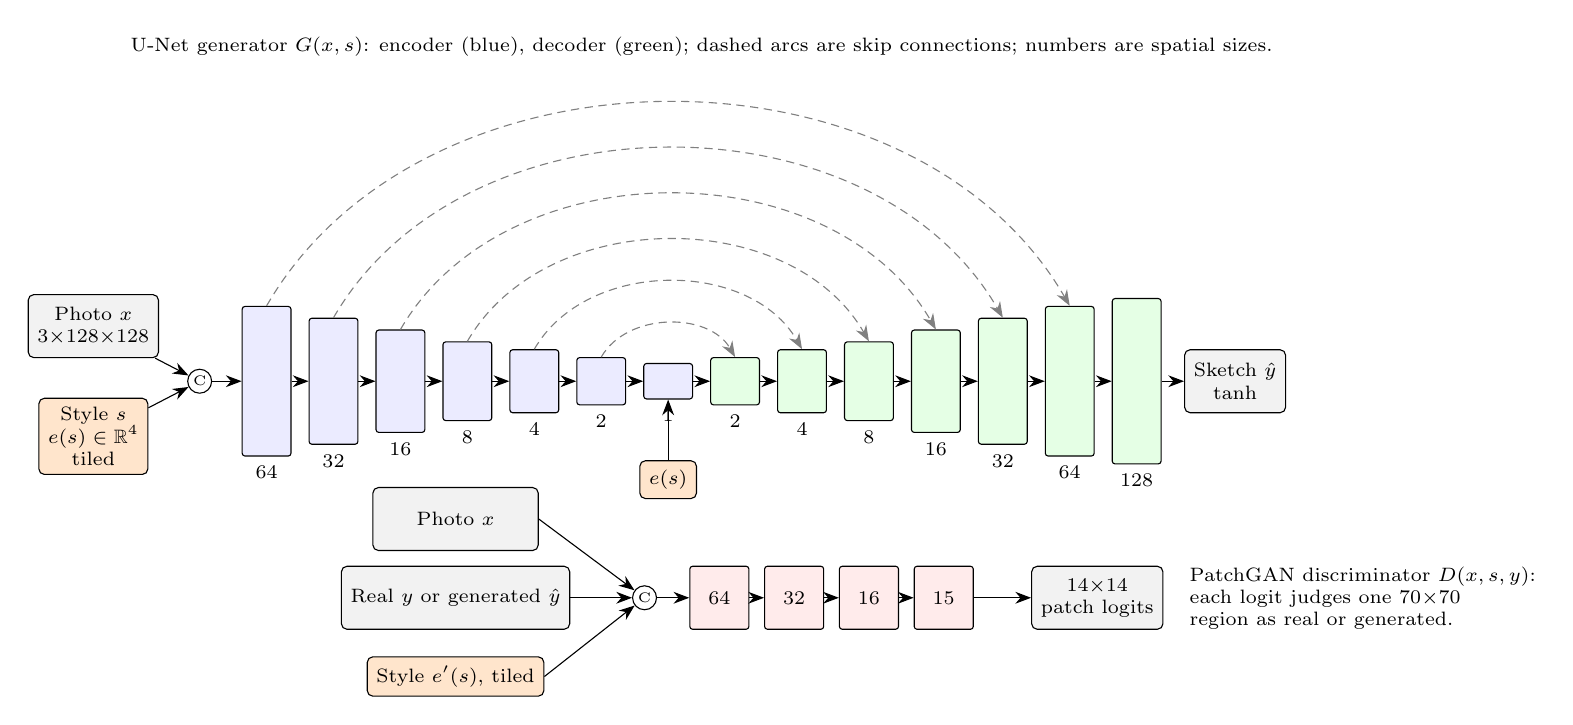
\begin{tikzpicture}[
  font=\scriptsize, >={Stealth[length=2mm]},
  blk/.style={draw, rounded corners=1pt, minimum width=0.62cm, align=center, fill=blue!8},
  dec/.style={draw, rounded corners=1pt, minimum width=0.62cm, align=center, fill=green!10},
  io/.style={draw, rounded corners=2pt, align=center, fill=gray!10, minimum height=0.8cm},
  emb/.style={draw, rounded corners=2pt, align=center, fill=orange!20},
  dsc/.style={draw, rounded corners=1pt, minimum width=0.75cm, align=center, fill=red!8}]
% generator input
\node[io] (x) at (0,0.7) {Photo $x$\\$3{\times}128{\times}128$};
\node[emb] (s) at (0,-0.7) {Style $s$\\$e(s)\in\mathbb{R}^{4}$\\tiled};
\node[draw, circle, inner sep=1pt] (cat1) at (1.35,0) {\tiny C};
\draw[->] (x) -- (cat1); \draw[->] (s) -- (cat1);
% encoder
\foreach \i/\h/\lab in {1/1.9/64, 2/1.6/32, 3/1.3/16, 4/1.0/8, 5/0.8/4, 6/0.6/2, 7/0.45/1}{
  \node[blk, minimum height=\h cm] (e\i) at ({1.35+0.85*\i},0) {};
  \node[below=0pt of e\i] {\lab};
}
\draw[->] (cat1) -- (e1);
\foreach \i [evaluate=\i as \j using int(\i+1)] in {1,...,6}{ \draw[->] (e\i) -- (e\j); }
% bottleneck style injection
\node[emb] (s2) at ({1.35+0.85*7},-1.25) {$e(s)$};
\draw[->] (s2) -- (e7.south);
% decoder
\foreach \i/\h/\lab in {1/0.6/2, 2/0.8/4, 3/1.0/8, 4/1.3/16, 5/1.6/32, 6/1.9/64, 7/2.1/128}{
  \node[dec, minimum height=\h cm] (d\i) at ({1.35+0.85*7+0.85*\i},0) {};
  \node[below=0pt of d\i] {\lab};
}
\draw[->] (e7) -- (d1);
\foreach \i [evaluate=\i as \j using int(\i+1)] in {1,...,6}{ \draw[->] (d\i) -- (d\j); }
% skips
\foreach \a/\b in {6/1, 5/2, 4/3, 3/4, 2/5, 1/6}{
  \draw[->, gray, densely dashed] (e\a.north) to[out=60, in=120] (d\b.north);
}
\node[io] (y) at ({1.35+0.85*14+1.25},0) {Sketch $\hat{y}$\\tanh};
\draw[->] (d7) -- (y);
\node[align=center] at ({1.35+0.85*7.5},4.25) {U-Net generator $G(x,s)$: encoder (blue), decoder (green); dashed arcs are skip connections; numbers are spatial sizes.};
% discriminator
\node[io, minimum width=2.1cm] (dx) at (4.6,-1.75) {Photo $x$};
\node[io, minimum width=2.1cm] (dy) at (4.6,-2.75) {Real $y$ or generated $\hat{y}$};
\node[emb, minimum width=2.1cm] (ds) at (4.6,-3.75) {Style $e'(s)$, tiled};
\node[draw, circle, inner sep=1pt] (cat2) at (7.0,-2.75) {\tiny C};
\draw[->] (dx.east) -- (cat2); \draw[->] (dy.east) -- (cat2); \draw[->] (ds.east) -- (cat2);
\foreach \i/\lab in {1/64, 2/32, 3/16, 4/15}{ \node[dsc, minimum height=0.8cm] (p\i) at ({7.0+0.95*\i},-2.75) {\lab}; }
\draw[->] (cat2) -- (p1); \draw[->] (p1) -- (p2); \draw[->] (p2) -- (p3); \draw[->] (p3) -- (p4);
\node[io] (out) at (12.75,-2.75) {$14{\times}14$\\patch logits};
\draw[->] (p4) -- (out);
\node[align=left, anchor=west] at (13.8,-2.75) {PatchGAN discriminator $D(x,s,y)$:\\each logit judges one $70{\times}70$\\region as real or generated.};
\end{tikzpicture}}
\caption{Task 4 architecture. The learned style embedding is tiled and concatenated (C) at the generator input and bottleneck, and the discriminator has its own style embedding at its input.}
\label{fig:t4_arch}
\end{figure*}

\subsection{Loss functions}
The discriminator is trained with binary cross-entropy on logits, real pairs labelled 1 and generated pairs labelled 0:
\begin{equation}
\mathcal{L}_{D} = \tfrac{1}{2}\bigl[\text{BCE}(D(x,s,y), 1) + \text{BCE}(D(x,s,G(x,s)), 0)\bigr].
\end{equation}
The factor $\tfrac{1}{2}$ slows the discriminator relative to the generator, as in pix2pix \cite{isola2017}. The generator uses the non-saturating adversarial loss plus an L1 reconstruction term:
\begin{equation}
\mathcal{L}_{G} = \text{BCE}(D(x,s,G(x,s)), 1) + \lambda_{L1}\, \mathcal{L}_{1}\bigl(y, G(x,s)\bigr).
\end{equation}
The adversarial term pushes the output towards realistic stroke texture, and the L1 term keeps it close to the paired ground truth. The commonly used value $\lambda_{L1} = 100$ \cite{isola2017} was the starting point; the final value was selected by Optuna. The discriminator real loss, discriminator fake loss, generator adversarial loss and generator L1 loss were logged separately at every epoch.

\subsection{Training procedure}
Weights were initialised from $\mathcal{N}(0, 0.02)$ and both networks were optimised with Adam \cite{kingma2015} using $\beta_1 = 0.5$, $\beta_2 = 0.999$, the setting recommended for stable GAN training \cite{radford2016}. Each iteration performs one discriminator update followed by one generator update. The final model was trained for 200 epochs: a constant learning rate for 100 epochs, then linear decay to zero, as in pix2pix. Validation metrics were computed every 5 epochs and the checkpoint with the best validation objective was kept. The same nine validation photographs (three per style) were generated every 10 epochs and logged to Weights \& Biases.

At inference the generator runs in evaluation mode, so dropout is disabled. Pix2pix keeps dropout active at test time as a source of variation \cite{isola2017}, but a deterministic output was preferred here so that the application gives the same sketch for the same photograph and the ONNX model can be verified exactly against PyTorch.

\subsection{Hyperparameter optimisation}
Optuna \cite{akiba2019} ran 16 trials of 20 epochs each with the TPE sampler \cite{bergstra2011} (seed 42) and a median pruner (4 start-up trials, no pruning before epoch 8), with validation every 4 epochs. Trial 0 was fixed to the standard pix2pix settings as a reference. The selection objective was
\begin{equation}
J = \text{LPIPS}_{\text{val}} + (1 - \text{SSIM}_{\text{val}}),
\end{equation}
which is fixed across trials and independent of $\lambda_{L1}$. LPIPS \cite{zhang2018lpips} rewards perceptual similarity of stroke texture and SSIM rewards facial structure. A pixel objective such as validation L1 was rejected because it would favour very large $\lambda_{L1}$ and therefore blurry sketches. Table~\ref{tab:t4_optuna} lists the search space.

\begin{table}[t]
\centering
\caption{Task 4 Optuna search space, pix2pix reference (trial 0) and best trial (trial 12).}
\label{tab:t4_optuna}
\footnotesize
\begin{tabular}{@{}llll@{}}
\toprule
Hyperparameter & Range & Trial 0 & Trial 12 \\
\midrule
Generator LR & log $[5\text{e-}5, 5\text{e-}4]$ & 2.0e-4 & 4.78e-4 \\
Discriminator LR & log $[2\text{e-}5, 5\text{e-}4]$ & 2.0e-4 & 3.79e-4 \\
Batch size & $\{4, 8, 16\}$ & 8 & 8 \\
Base channels $c$ & $\{32, 48, 64\}$ & 64 & 48 \\
Dropout & $[0, 0.5]$ & 0.50 & 0.43 \\
Style embedding $E$ & $\{4, 8, 16, 32\}$ & 8 & 4 \\
$\lambda_{L1}$ & log $[10, 200]$ & 100 & 23.3 \\
\midrule
Objective $J$ (20 epochs) & & 0.8308 & \textbf{0.8122} \\
\bottomrule
\end{tabular}
\end{table}

Eight trials completed and eight were pruned. The best trial (trial 12) reached $J = 0.8122$, against 0.8308 for the pix2pix reference. The four best completed trials (9, 10, 12 and 13) all used $c = 48$, batch size 8 and $E = 4$, and the two best both used $\lambda_{L1} \approx 23$. Optuna therefore preferred a much smaller L1 weight than the usual 100, which gives the adversarial term more influence over stroke texture. The two worst completed trials (2 and 3, $J = 1.016$ and 0.908) had the smallest discriminator learning rates ($3.6\times10^{-5}$ and $2.3\times10^{-5}$). A slowly learning discriminator gives the generator a weak adversarial signal, so the generator falls back on the L1 term and produces flatter sketches.

The fANOVA importances \cite{hutter2014} (Fig.~\ref{fig:t4_optuna}) assign 0.28 to the generator learning rate, 0.25 to $\lambda_{L1}$, 0.25 to dropout and 0.22 to the discriminator learning rate, and less than 0.01 to the categorical parameters. These estimates come from only eight completed trials, and the categorical parameters hardly varied among them, so their low importance means that the search did not resolve their effect rather than that they have none. The study was limited to 16 trials by GAN training cost; a longer search would make these estimates more reliable.

\begin{figure}[t]
\centering
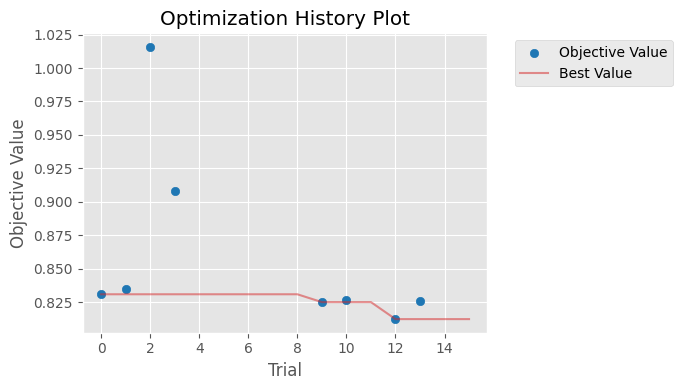
\includegraphics[width=0.92\linewidth]{t4_optuna_history.png}\\[2pt]
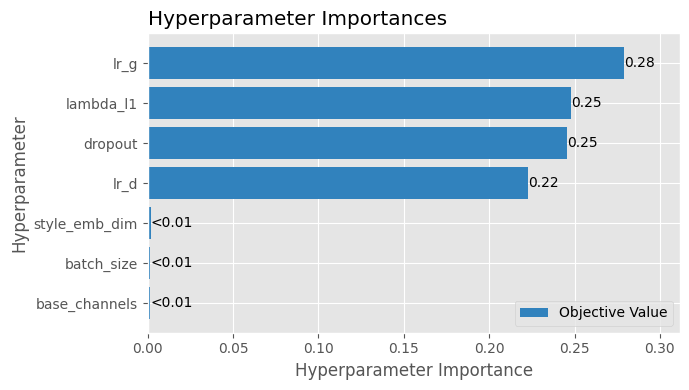
\includegraphics[width=0.92\linewidth]{t4_optuna_importance.png}
\caption{Task 4 Optuna results: objective per trial (top; pruned trials have no value) and fANOVA hyperparameter importance over completed trials (bottom).}
\label{fig:t4_optuna}
\end{figure}

\subsection{Training behaviour}
Fig.~\ref{fig:t4_curves} shows the separately logged losses for the final run. The generator L1 loss fell quickly from 0.30 to about 0.20 within 50 epochs and then decreased slowly to 0.191. Validation LPIPS dropped from 0.414 at epoch 5 to about 0.21 by epoch 50 and then levelled off near 0.20, while validation SSIM settled between 0.45 and 0.48. The validation objective was 0.7230 at epoch 100 and 0.7227 at epoch 200, so the second half of the schedule, with its decaying learning rate, refined the model only marginally. The selected checkpoint is from epoch 200.

The adversarial balance changed steadily during training. Both discriminator losses fell from about 0.6 to 0.19, the generator adversarial loss rose from about 1.1 to 2.3, and the discriminator patch accuracy on both real and generated sketches rose from about 0.70 to 0.96 (Fig.~\ref{fig:t4_dacc}). The discriminator therefore became increasingly confident. This did not damage the generator: validation SSIM and LPIPS did not deteriorate, because the L1 term keeps the generator anchored to the paired target. The short spikes in the discriminator loss before epoch 50 (with matching dips in the generator adversarial loss) were transient and recovered within a few epochs. A discriminator that wins this clearly does, however, supply less useful gradient late in training; one-sided label smoothing \cite{salimans2016}, spectral normalisation \cite{miyato2018sn} or a faster decay of the discriminator learning rate are possible remedies.

\begin{figure*}[t]
\centering
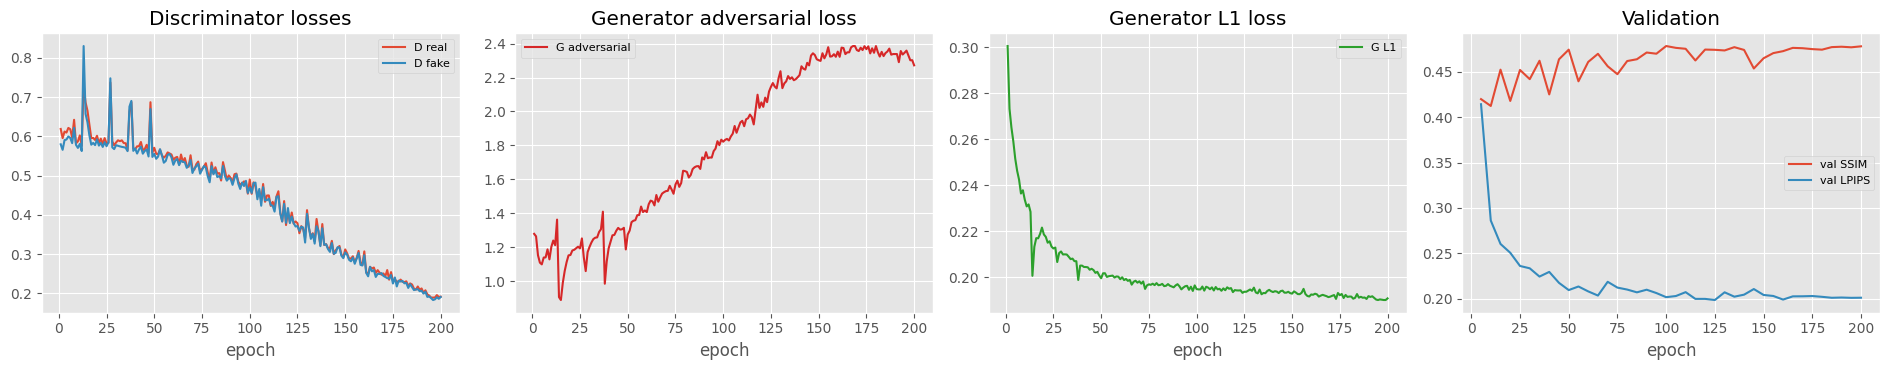
\includegraphics[width=\textwidth]{t4_training_curves.png}
\caption{Task 4 final training run: discriminator real and fake losses, generator adversarial loss, generator L1 loss, and validation SSIM and LPIPS (computed every 5 epochs).}
\label{fig:t4_curves}
\end{figure*}

\begin{figure}[t]
\centering
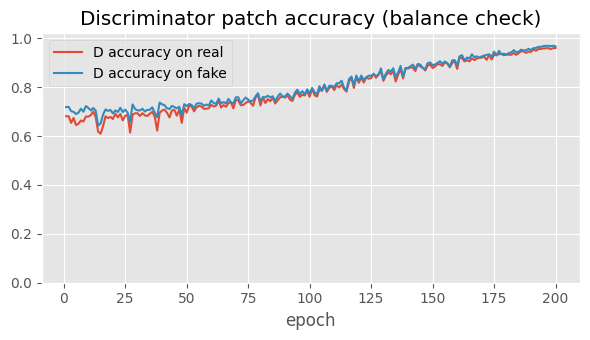
\includegraphics[width=0.85\linewidth]{t4_discriminator_accuracy.png}
\caption{Discriminator patch accuracy on real and generated sketches during the final run.}
\label{fig:t4_dacc}
\end{figure}

Fig.~\ref{fig:t4_time} shows the generator on fixed validation photographs. After one epoch the outputs are blurred blobs with a regular grid pattern, the checkerboard artefact typical of transposed convolutions early in training \cite{odena2016}. By epoch 40 the outputs are recognisable sketches with the correct overall tone for each style: light outlines for Style 1 and dark, heavily shaded hair for Style 2. Later epochs mainly sharpen strokes and facial details, and the differences between epochs 120 and 200 are small, which agrees with the validation plateau.

\begin{figure*}[t]
\centering
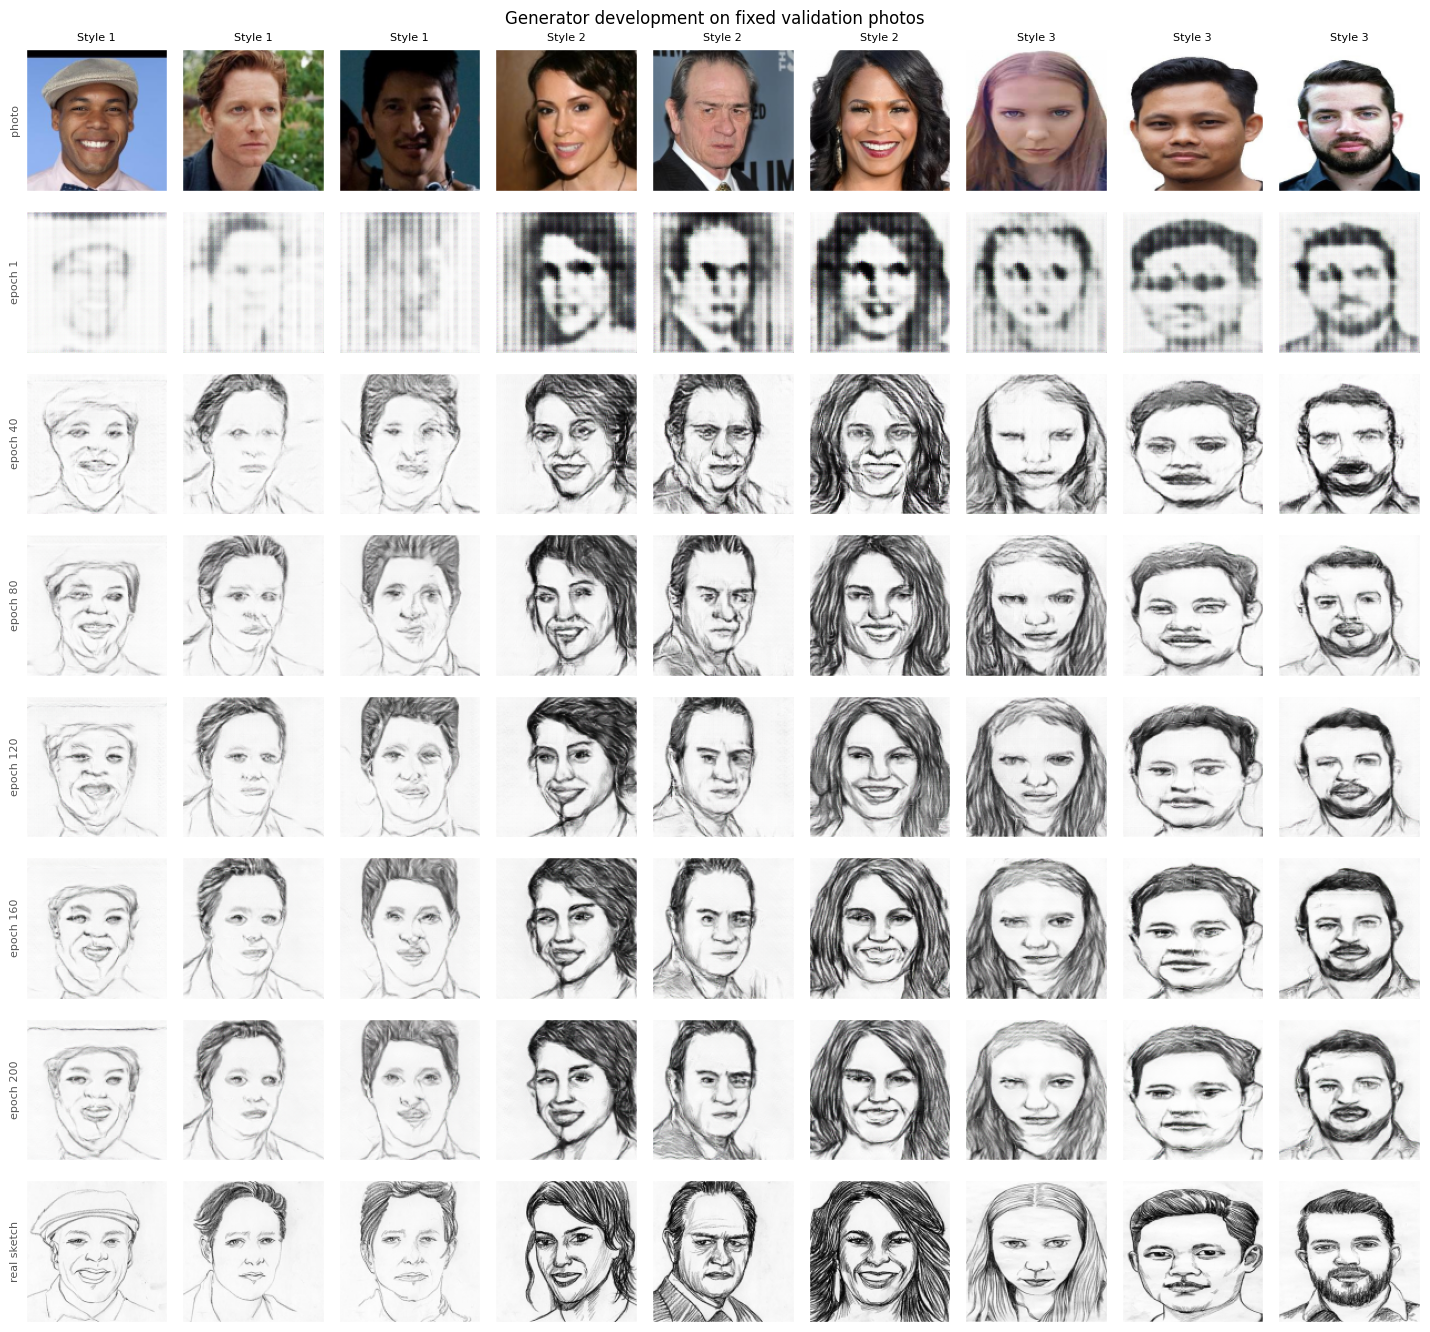
\includegraphics[width=0.82\textwidth]{t4_generator_over_time.png}
\caption{Generator development on nine fixed validation photographs (three per style). Top row: input; middle rows: output at selected epochs; bottom row: the artist's sketch.}
\label{fig:t4_time}
\end{figure*}

\subsection{Test results}
\label{sec:t4_results}
Each test photograph was generated with its true style. Table~\ref{tab:t4_test} reports pixel (L1, PSNR), structural (SSIM), perceptual (LPIPS) and distribution-level (FID, KID) metrics. FID and KID compare Inception features of all generated sketches with those of all real sketches \cite{heusel2017,binkowski2018}.

\begin{table}[t]
\centering
\caption{Task 4 results on the official FS2K test set (true style). Lower is better for L1, LPIPS, FID and KID.}
\label{tab:t4_test}
\footnotesize
\setlength{\tabcolsep}{3.5pt}
\begin{tabular}{@{}lrccccrc@{}}
\toprule
Subset & $n$ & L1 & PSNR & SSIM & LPIPS & FID & KID \\
\midrule
Overall & 1,046 & 0.107 & 15.54 & 0.463 & 0.211 & 37.6 & 0.030 \\
Style 1 & 619 & 0.082 & 17.24 & 0.504 & 0.214 & 42.3 & 0.033 \\
Style 2 & 381 & 0.152 & 12.46 & 0.380 & 0.211 & 46.8 & 0.040 \\
Style 3 & 46 & 0.069 & 18.10 & 0.591 & 0.164 & 80.3 & 0.046 \\
\bottomrule
\end{tabular}
\end{table}

Style 2 has by far the lowest PSNR and SSIM, yet its LPIPS (0.211) is as good as Style 1's. Style 2 sketches consist of dense, dark hatching (Fig.~\ref{fig:t4_data}); a hatching pattern that is perceptually correct but whose individual strokes are shifted by a few pixels is heavily penalised by pixel and structural metrics, but much less by a perceptual metric. Pixel metrics alone would therefore understate the quality of Style 2. Conversely, Style 3 has the best SSIM and LPIPS but the worst FID (80.3). FID is biased upwards for small samples \cite{chong2020}, and only 46 Style 3 test sketches are available, so this value mostly reflects sample size; KID, which is unbiased \cite{binkowski2018}, shows a much smaller gap (0.046 against 0.033 for Style 1). The KID standard deviation for Style 3 is zero only because all 46 images fit in a single KID subset. Because 59\% of the test set is Style 1, the overall figures are weighted towards that style.

\textbf{Does the style condition control the output?} Every test photograph was also generated in all three styles and compared with its real sketch (Table~\ref{tab:t4_style}). If the generator ignored the condition, the three outputs would be identical and match the real sketch equally well. Instead, the true style gives the lowest LPIPS for 72.9\% of Style 1, 90.8\% of Style 2 and 95.7\% of Style 3 photographs, and the three outputs for the same photograph differ by a mean absolute intensity of 0.095 to 0.115. The embedding therefore genuinely conditions the generator rather than acting as an interface label. Style 1 is separated least clearly: its closest competitor is Style 3 (LPIPS 0.235 against 0.214), which is consistent with both being lighter line styles, whereas Style 2 differs strongly from both.

\begin{table}[t]
\centering
\caption{Style control on the test set: LPIPS to the real sketch when each photograph is generated in each style (lower is better), and how often the true style is best.}
\label{tab:t4_style}
\footnotesize
\setlength{\tabcolsep}{4pt}
\begin{tabular}{@{}lrcccc@{}}
\toprule
True style & $n$ & as Style 1 & as Style 2 & as Style 3 & True style best \\
\midrule
Style 1 & 619 & \textbf{0.214} & 0.258 & 0.235 & 72.9\% \\
Style 2 & 381 & 0.294 & \textbf{0.211} & 0.242 & 90.8\% \\
Style 3 & 46 & 0.203 & 0.192 & \textbf{0.164} & 95.7\% \\
\bottomrule
\end{tabular}
\end{table}

\textbf{Qualitative results.} Fig.~\ref{fig:t4_rep} shows typical results (the test images closest to the median LPIPS of each style). The generator keeps identity, head shape, hairline and accessories such as glasses, and changing the style condition visibly changes stroke weight and shading in the expected direction. The main weaknesses are fine detail: generated hatching is simpler and more uniform than the artist's (most visible in Style 2 hair), eyes and mouths are sometimes softened, and thin glasses frames can be partly lost (fifth row).

\begin{figure}[t]
\centering
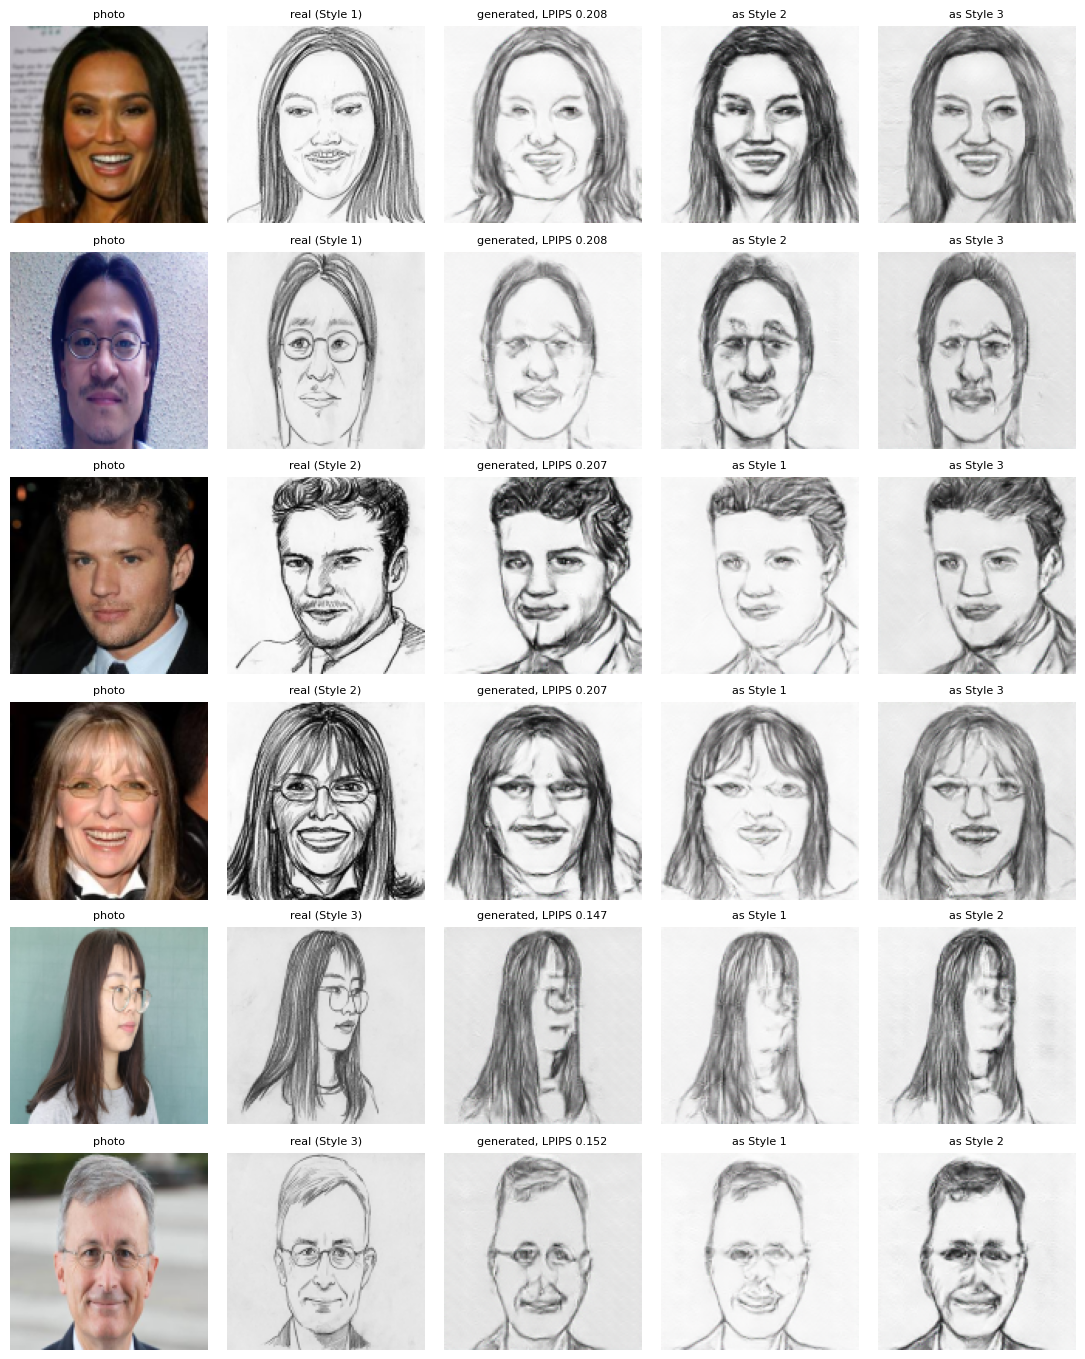
\includegraphics[width=\linewidth]{t4_representative_6rows.png}
\caption{Representative test results, two per style. Columns: photograph, real sketch, sketch generated with the true style, and the same photograph generated in the two other styles.}
\label{fig:t4_rep}
\end{figure}

\textbf{Failure cases.} Fig.~\ref{fig:t4_fail} shows the six test images with the highest LPIPS. All six are Style 1, whose sparse outlines make any extra stroke expensive, and they share a small set of causes. (i) Several faces in the frame (first two rows): the artist drew only the main subject, but the generator sketches every face and part of the background. (ii) A very dark, low-contrast photograph (third row): facial features cannot be recovered and the generator produces unstructured texture. (iii) A small subject in a wide scene with a detailed background (last row): background structures are drawn as strokes. (iv) Unusual colour casts and hairstyles (fourth and fifth rows): the hair shape is wrong and the face interior is under-drawn. In the first row the artist also omitted the head covering, so part of the error reflects artistic interpretation rather than a model mistake. FS2K faces are mostly centred and well lit, so these cases are out of distribution; a face detection and cropping step before inference would reduce them, and is relevant for webcam input in the application.

\begin{figure}[t]
\centering
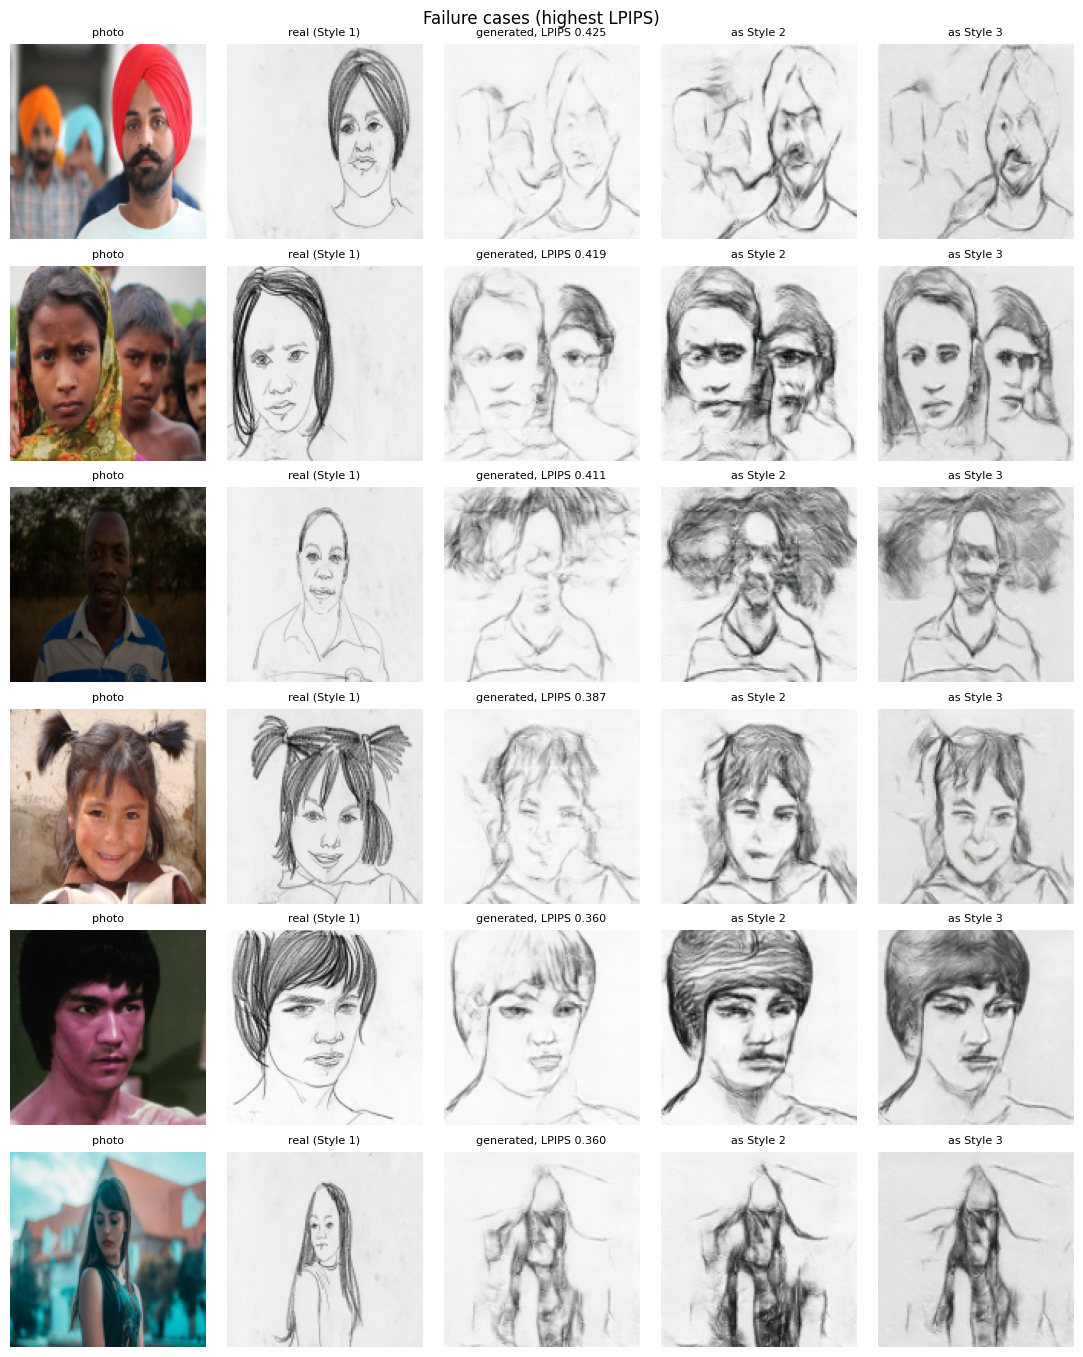
\includegraphics[width=\linewidth]{t4_failure_cases.png}
\caption{Task 4 failure cases (highest test LPIPS): multiple faces, very dark lighting, unusual colour and hairstyles, and a small subject in a busy scene.}
\label{fig:t4_fail}
\end{figure}

\subsection{ONNX export}
Only the generator is exported; the discriminator is a training component. A wrapper converts inputs from $[0,1]$ to $[-1,1]$ and outputs back to $[0,1]$, so the ONNX model (opset 17, dynamic batch size) takes \texttt{photo} ($N{\times}3{\times}128{\times}128$, RGB in $[0,1]$) and \texttt{style} ($N$, int64 in $\{0,1,2\}$) and returns \texttt{sketch} in $[0,1]$. On 60 test photographs, the maximum absolute difference between ONNX Runtime and PyTorch was $1.6\times10^{-6}$, $2.7\times10^{-6}$ and $1.8\times10^{-6}$ for the three styles, which is within floating-point tolerance. The model file is 94.3\,MB, and the mean CPU latency for one image in ONNX Runtime was 25.5\,ms (95th percentile 29.7\,ms) on the Colab CPU.

% =====================================================================
\section{Application Design and Deployment}

\subsection{Interface design}
The interface was first designed in Google Stitch from a written specification (Fig.~\ref{fig:stitch_canvas}), which produced the four workspace screens in Fig.~\ref{fig:stitch}. The design goals were a calm, minimal interface for an evaluator who uploads an image, runs a model and inspects the output together with system information. The palette is a lavender-tinted white page, baby blue control panels and lavender accents, with a deeper lavender for primary buttons and slate navy instead of black for text; a single rounded typeface (Nunito) is used throughout. Every screen shares one structure: a sidebar listing the four workspaces with a status dot (ready or coming soon) and a server status box, then the workspace title, a one-sentence description, a control panel on the left and the results area on the right. The Stitch screens for Hard-Routed and Soft Mixture-of-Experts Restoration introduced the probability and routing-weight bars with the selected branch highlighted, which the implementation adopted. The implementation simplified some Stitch details: decorative labels and invented system figures (for example GPU cluster statistics) were replaced by real values reported by the backend.

\begin{figure}[t]
\centering

\includegraphics[width=\linewidth]{stitch_canvas.png}
\caption{The Google Stitch project: the design prompt (bottom left) and the generated screens on the canvas.}
\label{fig:stitch_canvas}
\end{figure}

\begin{figure*}[t]
\centering
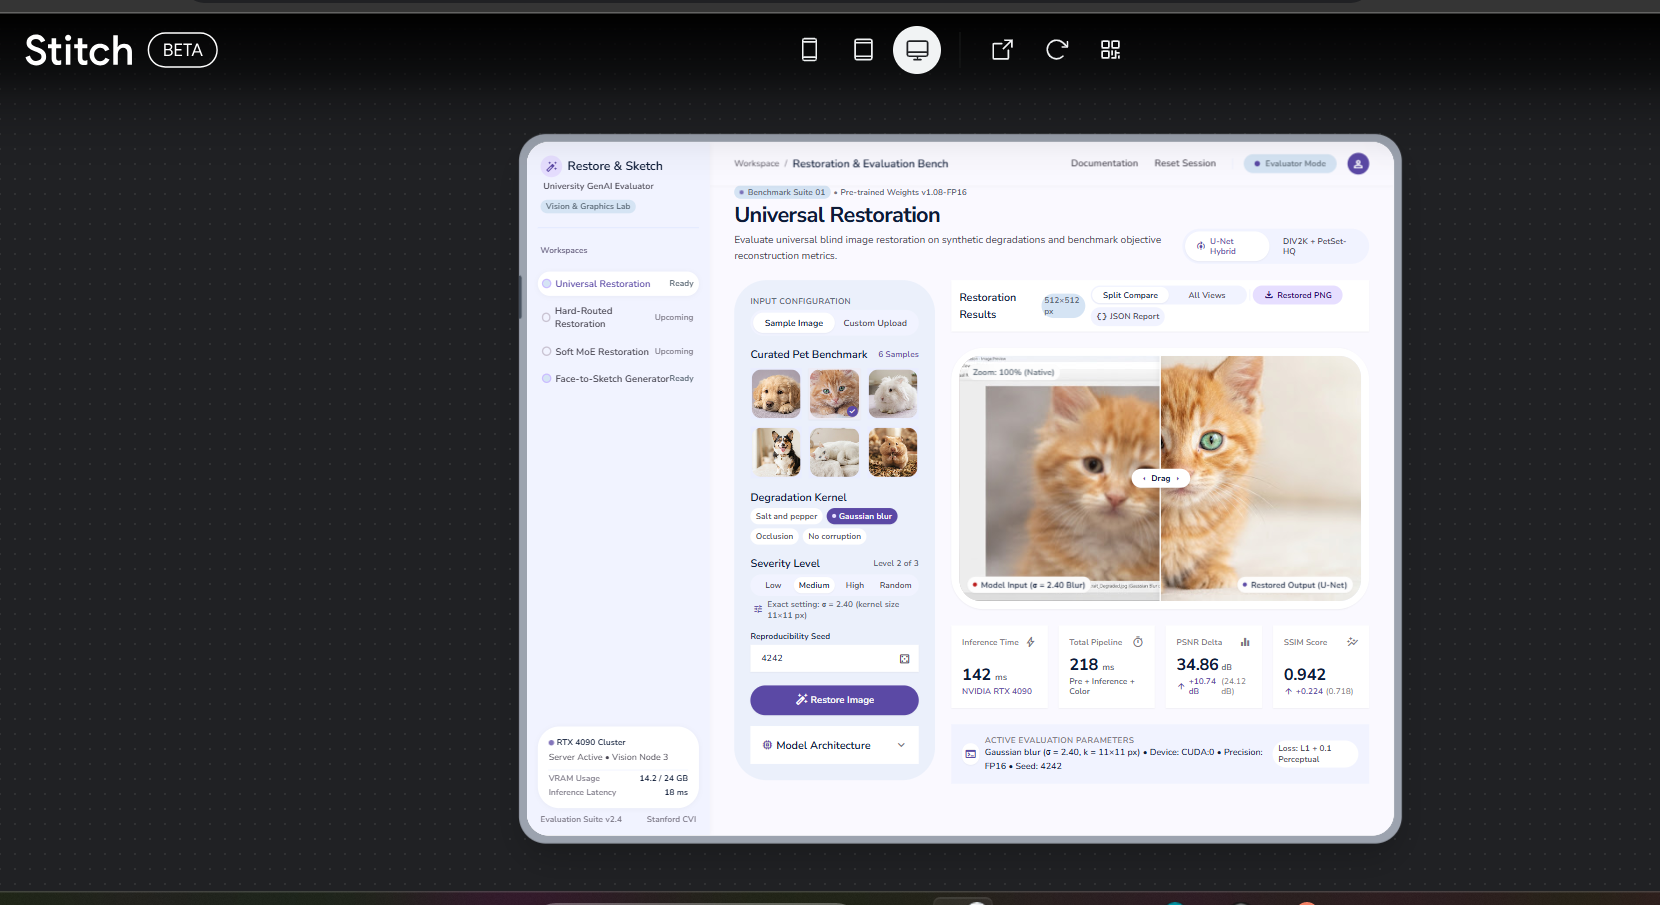
\includegraphics[width=0.49\textwidth]{stitch_universal.png}\hfill

\includegraphics[width=0.49\textwidth]{stitch_hard.png}\\[4pt]

\includegraphics[width=0.49\textwidth]{stitch_soft.png}\hfill

\includegraphics[width=0.49\textwidth]{stitch_sketch.png}
\caption{Original Google Stitch designs of the four workspaces: Universal Restoration, Hard-Routed Restoration, Soft Mixture-of-Experts Restoration and Face-to-Sketch Generator.}
\label{fig:stitch}
\end{figure*}

\subsection{System architecture}
Fig.~\ref{fig:sysarch} shows the deployed system. The frontend is a React single-page application styled with Tailwind CSS, built with Vite and served by nginx. nginx also forwards every request under \texttt{/api} to the FastAPI backend, so the browser talks to a single address. The backend loads every ONNX model once at start-up into an ONNX Runtime CPU session. A task whose files are missing is reported as unavailable instead of stopping the server. For each request the backend validates the upload (format, size, readability), converts it to RGB, applies the same preprocessing as in training (bicubic resizing for Tasks 1 and 2, area resizing for Task 4), runs the model and returns the images as PNG data together with timings and the relevant model outputs. The corruption code is the unchanged Task 1 module, so corruptions applied in the application are identical to those used in training and in the test manifest. The PSNR and SSIM shown in the interface use the training definitions, and the backend's SSIM was checked to agree with the training implementation to five decimal places.

\begin{figure}[t]
\centering
\resizebox{\linewidth}{!}{%
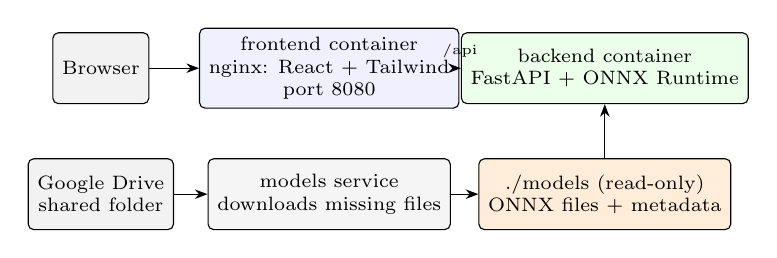
\begin{tikzpicture}[font=\scriptsize, >={Stealth[length=1.6mm]},
  box/.style={draw, rounded corners=2pt, align=center, minimum height=0.9cm, fill=white}]
\node[box, fill=gray!10] (br) at (0,0) {Browser};
\node[box, fill=blue!6] (fe) at (2.9,0) {frontend container\\nginx: React + Tailwind\\port 8080};
\node[box, fill=green!8] (be) at (6.4,0) {backend container\\FastAPI + ONNX Runtime};
\node[box, fill=orange!15] (md) at (6.4,-1.6) {./models (read-only)\\ONNX files + metadata};
\node[box, fill=gray!8] (mf) at (2.9,-1.6) {models service\\downloads missing files};
\node[box, fill=gray!10] (gd) at (0,-1.6) {Google Drive\\shared folder};
\draw[->] (br) -- (fe); \draw[->] (fe) -- node[above]{\tiny /api} (be);
\draw[->] (md) -- (be); \draw[->] (gd) -- (mf); \draw[->] (mf) -- (md);
\end{tikzpicture}}
\caption{Deployment: three Docker Compose services. The models service runs first and downloads any missing model file; the backend serves the API; nginx serves the interface and forwards API calls.}
\label{fig:sysarch}
\end{figure}

\begin{table}[t]
\centering
\caption{Backend endpoints (interactive documentation at \texttt{/api/docs}).}
\label{tab:api}
\footnotesize
\begin{tabular}{@{}p{2.9cm}p{4.9cm}@{}}
\toprule
Endpoint & Purpose \\
\midrule
GET /api/health & Server status, ONNX Runtime version, status of each model \\
GET /api/models & Per model: ONNX files, inputs, outputs, size, configuration, load time \\
GET /api/samples & Clean Oxford-IIIT Pet test images for the sample picker \\
POST /api/universal/restore & Task 1: image or sample, corruption, severity, seed; returns input, restoration, clean target, error map, PSNR, SSIM, settings, timings \\
POST /api/hard-routing/restore & Task 2: as Task 1, plus routing mode (classifier or oracle); returns the four probabilities, predicted class, branch used, correctness, and classifier and expert timings \\
POST /api/soft-moe/restore & Task 3: as Task 1; returns the four routing weights, strongest and contributing branches, routing entropy, restoration, scores and timings \\
POST /api/sketch & Task 4: photograph and style (1, 2 or 3), optionally all styles; returns the sketch at 128 and 512 pixels and timings \\
\bottomrule
\end{tabular}
\end{table}

\subsection{Workspaces}
\textbf{Universal Restoration} lets the user choose a clean sample image or upload one, apply a corruption at a fixed test severity (low, medium, high) or a random training-range severity, optionally with a fixed seed, or upload an already corrupted image unchanged. The result is shown in a before-and-after comparison slider or as a grid with the clean target and the error map, together with inference time, total server time, PSNR and SSIM before and after restoration, and every corruption setting used. Images are displayed pixel-sharp at their true 128$\times$128 resolution, so the evaluator sees exactly what the model received and produced.

\textbf{Hard-Routed Restoration} uses the same inputs and adds a routing switch: classifier (predicted) routing, or oracle routing by the known corruption when the application applied it. It shows the four classifier probabilities as bars, marks the predicted class, the true corruption and the branch that actually ran, states in plain words whether the classifier was correct and whether an expert was run or the identity bypass was used, and reports classifier and specialist time separately.

\textbf{Soft Mixture-of-Experts Restoration} uses the same inputs and shows the four routing weights as bars. The strongest branch is highlighted, and every branch with at least 10\% weight is marked as a contributor. A sentence states whether one branch dominated or the result is a blend, and the panel also reports the routing entropy, the restoration with its quality scores and the inference time of the complete ONNX pipeline (gate and all experts).

\textbf{Face-to-Sketch Generator} accepts an uploaded photograph or a webcam capture (centre-cropped to a square), offers Style 1, 2 or 3, and shows the photograph and the generated sketch side by side, with an option to draw all three styles for comparison. The sketch can be downloaded at the model's 128-pixel resolution or upscaled to 512 pixels.

\IfFileExists{figures/app_universal.png}{%
\begin{figure*}[t]
\centering
\includegraphics[width=0.49\textwidth]{app_universal.png}\hfill
\includegraphics[width=0.49\textwidth]{app_hard.png}\\[4pt]
\includegraphics[width=0.49\textwidth]{app_soft.png}\hfill
\includegraphics[width=0.49\textwidth]{app_sketch.png}
\caption{The four workspaces of the implemented application: Universal Restoration, Hard-Routed Restoration, Soft Mixture-of-Experts Restoration and Face-to-Sketch Generator.}
\label{fig:app_screens}
\end{figure*}}{}

\subsection{Containerised deployment}
The application runs as three Docker Compose services (Fig.~\ref{fig:sysarch}). The backend image is based on \texttt{python:3.12-slim} with pinned versions of FastAPI, ONNX Runtime, NumPy, OpenCV and Pillow, and has a health check on \texttt{/api/health}. The frontend image is built in two stages: Node 20 builds the React application, and the result is copied into an \texttt{nginx:1.27-alpine} image. A short-lived models service runs first. It checks the \texttt{models} folder and, if any file is missing, downloads the shared Google Drive folder whose address is stored in the repository's \texttt{.env} file. A failed download is reported but does not block the application, and model files are never stored in the Git repository. The whole system starts with the single command \texttt{docker compose up --build}, after which the application is available at \texttt{http://localhost:8080}. For GitHub Codespaces, where Docker's internal network can be unavailable, an override file runs the same services on the host network and is started with \texttt{./codespaces-up.sh}.

\subsection{Experiment tracking and reproducibility}
All Optuna trials, final training runs, separately logged losses, validation sample grids, result tables, checkpoints and ONNX files were recorded in Weights \& Biases (project \texttt{genai-assignment1}), grouped by task and by stage (Optuna trials, final training, test and export). Data splits, corruption manifests and Optuna studies are stored in the repository so that every experiment can be repeated.

\IfFileExists{figures/wandb.png}{\begin{figure}[t]\centering\includegraphics[width=\linewidth]{wandb.png}\caption{Weights \& Biases project with the runs of all four tasks.}\label{fig:wandb}\end{figure}}{}

% =====================================================================
\section{Limitations}
For Tasks 1 and 2: (i) the bottleneck limits output quality to about SSIM 0.73 regardless of the input, so mild blur and low-coverage occlusion are made worse by restoration; (ii) outputs are smoothed and strongly desaturated, and highly textured scenes fail; (iii) the skip-connection ablation showed that a narrow skip would add about 0.11 SSIM, a gain deliberately not taken in order to keep a strict bottleneck; (iv) the final Task 1 model and the specialists were still improving at the end of their schedules; (v) only three corruption types, one at a time, at 128$\times$128 were studied; and (vi) the classifier confuses clean photographs that contain large black regions or are naturally soft with occlusion and blur. For Task 3: (vii) the weak classification constraint selected by Optuna turned the gate into a mixer that is dominated by the identity branch, leaves the blur expert almost unused and keeps light occlusion boxes in place; (viii) blending produces ghosting such as semi-transparent boxes and residual noise; and (ix) every expert runs for every image, so inference costs about four times as much as hard routing.
For Task 4: (i) the test set contains only 46 Style 3 pairs, so per-style statistics for Style 3, especially FID, are uncertain; (ii) the Optuna study used 16 short trials, so hyperparameter importances are only indicative; (iii) the discriminator became dominant late in training, which limits further gains from the adversarial term; (iv) generated hatching is simpler than the artists' strokes at 128$\times$128; and (v) photographs unlike FS2K (several faces, poor lighting, small faces, webcam framing) produce poor sketches without a face detection and cropping step.

% =====================================================================
\section{Conclusion}
For restoration, a single autoencoder with a 12:1 bottleneck (Task 1) removed salt-and-pepper noise well but reached the same quality ceiling, about SSIM 0.73, for every input, and so degraded clean and mildly corrupted images. Hard routing (Task 2) worked almost perfectly as a routing mechanism: the classifier reached 99.86\% test accuracy, and predicted routing matched oracle routing. Its main benefit was the identity bypass, which keeps clean images intact and raised overall test SSIM from 0.704 to 0.735, while specialisation allowed a four-times smaller code at equal quality. The remaining routing errors showed that leaving lightly corrupted images untouched can beat any restoration, which motivated the weighted identity branch of Task 3. The jointly trained soft mixture of experts (Task 3) turned this observation into a learned policy: its gate keeps clean images and lightly damaged images largely unchanged, sends noise to the noise expert, and moves weight from the identity branch to the matching expert as blur and occlusion become more severe. This raised validation SSIM from 0.783 to 0.839, at the cost of running every expert for every image, an almost unused blur expert and visible blending artefacts. Across the three strategies, a shared model is simplest but degrades easy inputs; hard routing adds reliable, cheap specialisation; and soft routing gives the best scores by deciding how much to restore, though optimising SSIM alone sometimes prefers leaving visible damage in place.
For Task 4, a pix2pix-style conditional GAN with a learned style embedding in both the generator and the discriminator produced sketches that preserve identity and follow the requested style, with a test LPIPS of 0.211 and FID of 37.6. The style-control experiment showed that the embedding changes the output in the intended direction, especially for the visually distinctive Styles 2 and 3. Hyperparameter optimisation favoured a much lower L1 weight than the standard pix2pix setting, and pixel metrics proved misleading for heavily hatched styles, which supports using perceptual and distribution-level metrics for sketch synthesis.

% =====================================================================
\section*{Code, Models and Video}
Repository: \url{https://github.com/eman-huda/genai-assignment1}. The trained ONNX models are not stored in the repository; Docker Compose downloads them automatically from the shared folder configured in the repository's \texttt{.env} file, as described in its README. \videosentence

% =====================================================================
\begin{thebibliography}{99}
\bibitem{vincent2008} P. Vincent, H. Larochelle, Y. Bengio and P.-A. Manzagol, ``Extracting and composing robust features with denoising autoencoders,'' in \emph{Proc. ICML}, 2008, pp. 1096--1103.
\bibitem{mao2016} X. Mao, C. Shen and Y.-B. Yang, ``Image restoration using very deep convolutional encoder-decoder networks with symmetric skip connections,'' in \emph{Proc. NeurIPS}, 2016.
\bibitem{zhang2017dncnn} K. Zhang, W. Zuo, Y. Chen, D. Meng and L. Zhang, ``Beyond a Gaussian denoiser: Residual learning of deep CNN for image denoising,'' \emph{IEEE Trans. Image Process.}, vol. 26, no. 7, pp. 3142--3155, 2017.
\bibitem{pathak2016} D. Pathak, P. Kr\"ahenb\"uhl, J. Donahue, T. Darrell and A. A. Efros, ``Context encoders: Feature learning by inpainting,'' in \emph{Proc. CVPR}, 2016, pp. 2536--2544.
\bibitem{li2022airnet} B. Li, X. Liu, P. Hu, Z. Wu, J. Lv and X. Peng, ``All-in-one image restoration for unknown corruption,'' in \emph{Proc. CVPR}, 2022, pp. 17452--17462.
\bibitem{jacobs1991} R. A. Jacobs, M. I. Jordan, S. J. Nowlan and G. E. Hinton, ``Adaptive mixtures of local experts,'' \emph{Neural Comput.}, vol. 3, no. 1, pp. 79--87, 1991.
\bibitem{shazeer2017} N. Shazeer \emph{et al.}, ``Outrageously large neural networks: The sparsely-gated mixture-of-experts layer,'' in \emph{Proc. ICLR}, 2017.
\bibitem{fedus2022} W. Fedus, B. Zoph and N. Shazeer, ``Switch transformers: Scaling to trillion parameter models with simple and efficient sparsity,'' \emph{J. Mach. Learn. Res.}, vol. 23, no. 120, pp. 1--39, 2022.
\bibitem{goodfellow2014} I. Goodfellow \emph{et al.}, ``Generative adversarial nets,'' in \emph{Proc. NeurIPS}, 2014, pp. 2672--2680.
\bibitem{mirza2014} M. Mirza and S. Osindero, ``Conditional generative adversarial nets,'' arXiv:1411.1784, 2014.
\bibitem{ronneberger2015} O. Ronneberger, P. Fischer and T. Brox, ``U-Net: Convolutional networks for biomedical image segmentation,'' in \emph{Proc. MICCAI}, 2015, pp. 234--241.
\bibitem{isola2017} P. Isola, J.-Y. Zhu, T. Zhou and A. A. Efros, ``Image-to-image translation with conditional adversarial networks,'' in \emph{Proc. CVPR}, 2017, pp. 1125--1134.
\bibitem{wang2009} X. Wang and X. Tang, ``Face photo-sketch synthesis and recognition,'' \emph{IEEE Trans. Pattern Anal. Mach. Intell.}, vol. 31, no. 11, pp. 1955--1967, 2009.
\bibitem{fan2022} D.-P. Fan, Z. Huang, P. Zheng, H. Liu, X. Qin and L. Van Gool, ``Facial-sketch synthesis: A new challenge,'' \emph{Mach. Intell. Res.}, vol. 19, no. 4, pp. 257--287, 2022.
\bibitem{miyato2018proj} T. Miyato and M. Koyama, ``cGANs with projection discriminator,'' in \emph{Proc. ICLR}, 2018.
\bibitem{wang2004} Z. Wang, A. C. Bovik, H. R. Sheikh and E. P. Simoncelli, ``Image quality assessment: From error visibility to structural similarity,'' \emph{IEEE Trans. Image Process.}, vol. 13, no. 4, pp. 600--612, 2004.
\bibitem{zhang2018lpips} R. Zhang, P. Isola, A. A. Efros, E. Shechtman and O. Wang, ``The unreasonable effectiveness of deep features as a perceptual metric,'' in \emph{Proc. CVPR}, 2018, pp. 586--595.
\bibitem{heusel2017} M. Heusel, H. Ramsauer, T. Unterthiner, B. Nessler and S. Hochreiter, ``GANs trained by a two time-scale update rule converge to a local Nash equilibrium,'' in \emph{Proc. NeurIPS}, 2017.
\bibitem{chong2020} M. J. Chong and D. Forsyth, ``Effectively unbiased FID and Inception Score and where to find them,'' in \emph{Proc. CVPR}, 2020, pp. 6070--6079.
\bibitem{binkowski2018} M. Bi\'nkowski, D. J. Sutherland, M. Arbel and A. Gretton, ``Demystifying MMD GANs,'' in \emph{Proc. ICLR}, 2018.
\bibitem{akiba2019} T. Akiba, S. Sano, T. Yanase, T. Ohta and M. Koyama, ``Optuna: A next-generation hyperparameter optimization framework,'' in \emph{Proc. ACM SIGKDD}, 2019, pp. 2623--2631.
\bibitem{bergstra2011} J. Bergstra, R. Bardenet, Y. Bengio and B. K\'egl, ``Algorithms for hyper-parameter optimization,'' in \emph{Proc. NeurIPS}, 2011.
\bibitem{hutter2014} F. Hutter, H. Hoos and K. Leyton-Brown, ``An efficient approach for assessing hyperparameter importance,'' in \emph{Proc. ICML}, 2014, pp. 754--762.
\bibitem{parkhi2012} O. M. Parkhi, A. Vedaldi, A. Zisserman and C. V. Jawahar, ``Cats and dogs,'' in \emph{Proc. CVPR}, 2012, pp. 3498--3505.
\bibitem{kingma2015} D. P. Kingma and J. Ba, ``Adam: A method for stochastic optimization,'' in \emph{Proc. ICLR}, 2015.
\bibitem{radford2016} A. Radford, L. Metz and S. Chintala, ``Unsupervised representation learning with deep convolutional generative adversarial networks,'' in \emph{Proc. ICLR}, 2016.
\bibitem{salimans2016} T. Salimans \emph{et al.}, ``Improved techniques for training GANs,'' in \emph{Proc. NeurIPS}, 2016.
\bibitem{miyato2018sn} T. Miyato, T. Kataoka, M. Koyama and Y. Yoshida, ``Spectral normalization for generative adversarial networks,'' in \emph{Proc. ICLR}, 2018.
\bibitem{odena2016} A. Odena, V. Dumoulin and C. Olah, ``Deconvolution and checkerboard artifacts,'' \emph{Distill}, 2016.
\end{thebibliography}

% =====================================================================
\appendices
\section{AI Use}
\label{app:ai}
Generative AI tools were used as permitted by the assignment. All generated code was run, tested and checked, and all generated text was reviewed against the actual results. Table~\ref{tab:ai_use} lists each use.

\begin{table*}[t]
\centering
\caption{Use of AI tools and how their outputs were verified.}
\label{tab:ai_use}
\footnotesize
\begin{tabular}{@{}p{2.2cm}p{5.2cm}p{8.8cm}@{}}
\toprule
Tool & Used for & Verification and corrections \\
\midrule
Claude (Anthropic) & Task 1 notebook and shared code (corruptions, data, model, training, evaluation, ONNX export) & Corruption definitions were checked against the brief and inspected visually (Fig.~\ref{fig:corruption_examples}); the achieved occlusion coverage and the balanced validation manifest were verified from printed statistics; ONNX outputs matched PyTorch within $7.2\times10^{-7}$. \\
Claude (Anthropic) & Task 2 notebook (classifier, balanced sampler, specialists, hard routing, ONNX export) & The balanced batches were verified by printing class counts per batch; ONNX outputs matched PyTorch (identical predicted classes); oracle and predicted routing were compared on the full test set. \\
Claude (Anthropic) & Task 3 notebook (soft MoE model, balanced sampler, joint training, routing analysis, ONNX export) & The loaded Task 2 components were checked to reproduce the Task 2 validation results before training; routing weights were checked for collapse during the search; warm-up freezing, balanced batches and weight normalisation were verified in tests. \\
Claude (Anthropic) & Task 4 notebook, shared modules and command-line scripts (FS2K pairing, paired augmentation, U-Net and PatchGAN with style embedding, training, evaluation, ONNX export) & Code was smoke-tested on a synthetic dataset with the FS2K folder layout before use. On the real data: the pairing report showed 0 missing pairs and 0 size mismatches; the paired augmentation figure was inspected for alignment; ONNX outputs matched PyTorch within $3\times10^{-6}$ for all styles; training curves, generated samples and failure cases were inspected manually. \\
Claude (Anthropic) & Web application (FastAPI backend, React and Tailwind frontend, Docker Compose) & Every endpoint was tested with valid and invalid requests; the backend SSIM was checked against the training implementation; the application was run end to end in GitHub Codespaces. \\
Claude (Anthropic) & Drafting the Task 1 to 4 sections and the application section of this report from the executed notebook outputs & All numbers were checked against the notebook outputs and the interpretations against the figures. The text was reviewed by the author. \\
Google Stitch & Interface design from a written prompt & The generated screens were compared with the implementation; invented figures in the design were replaced by real backend values. \\
\bottomrule
\end{tabular}
\end{table*}

\end{document}
